\documentclass[12pt]{article}
\usepackage[spanish,mexico]{babel}
	\selectlanguage{spanish}
\usepackage{graphicx}
\usepackage{amsmath}
\usepackage{wrapfig}
\usepackage{color}
\usepackage[dvipsnames]{xcolor}
\usepackage{float}
\usepackage{multicol}
\usepackage{geometry}
\usepackage{hyperref}
\usepackage[utf8]{inputenc}

\newgeometry{top=2cm}
\definecolor{labelcolor}{RGB}{100,0,0}

\title{Actividad 8: Iniciándose en cómputo simbólico con Maxima}
\author{Ana Gabriela Carretas Talamante}
\date{15 de abril de 2016}

\begin{document}
\maketitle
\section{Introducción}
En esta actividad se nos presentó una herramienta de cálculo bastante versátil:Maxima. Es un sistema para la manipulación de expresiones simbólicas y numéricas, incluyendo diferenciación, integración, expansión en series de Taylor, transformadas de Laplace, ecuaciones diferenciales ordinarias, sistemas de ecuaciones lineales, vectores, matrices y tensores. Maxima produce resultados de alta precisión usando fracciones exactas, números enteros de precisión arbitraria y números de coma flotante con precisión variable. Adicionalmente puede graficar funciones y datos en dos y tres dimensiones \cite{M}.

\begin{figure}[H]
\centering
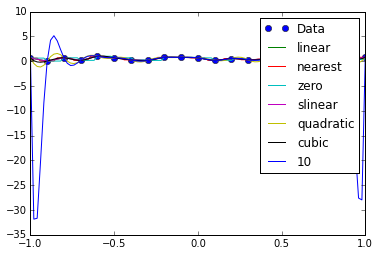
\includegraphics[width=10cm]{1}
\caption{Interfaz de trabajo en Maxima}
\end{figure}

Se nos pidió familiarizarnos con esta herramienta de cálculo al basarnos en el manual de Jay Kerns sobre cálculo en varias variables utilizando Maxima \cite{JK}. En esta ocasión trabajé en wxMaxima, un programa que permite visualizar gráficamente los comandos utilizados en Maxima para mayor comodidad. De ahí exporté los códigos en formato \texttt{.tex} para incluirlos en la bitácora presentada a continuación.

\section{Bitácora de trabajo}
\subsection{Geometría en tres dimensiones}
\paragraph{Vectores y álgebra lineal} En esta sección aprendimos a declarar vectores y algunas de las operaciones básicas entre ellos, como el producto punto y el producto cruz.

\noindent
\begin{minipage}[t]{8ex}{\color{red}\bf
\begin{verbatim}
(%i1) 
\end{verbatim}}
\end{minipage}
\begin{minipage}[t]{\textwidth}{\color{blue}
\begin{verbatim}
a: [4,3,-5];
b: [0,-1,7];
c: [-2,-6,-1];
d: (a.b)/(a.c);
load(vect);
b.(a~c);
express(\%);
\end{verbatim}}
\end{minipage}
\begin{math}\displaystyle
\parbox{8ex}{\color{labelcolor}(\%o1) }
[4,3,-5]
\end{math}

\noindent
\begin{math}\displaystyle
\parbox{8ex}{\color{labelcolor}(\%o2) }
[0,-1,7]
\end{math}

\noindent
\begin{math}\displaystyle
\parbox{8ex}{\color{labelcolor}(\%o3) }
[-2,-6,-1]
\end{math}

\noindent
\begin{math}\displaystyle
\parbox{8ex}{\color{labelcolor}(\%o4) }
\frac{38}{21}
\end{math}

\noindent
\begin{math}\displaystyle
\parbox{8ex}{\color{labelcolor}(\%o6) }
-[0,-1,7] . [-2,-6,-1]~[4,3,-5]
\end{math}

\noindent
\begin{math}\displaystyle
\parbox{8ex}{\color{labelcolor}(\%o7) }
-140
\end{math}

\paragraph{Líneas, planos y superficies cuadráticas} Definimos ecuaciones de planos y superficies, para poder visualizarlas en una imagen.

\noindent
\begin{minipage}[t]{8ex}{\color{red}\bf
\begin{verbatim}
(%i19) 
\end{verbatim}}
\end{minipage}
\begin{minipage}[t]{\textwidth}{\color{blue}
\begin{verbatim}
load(draw);
cosa: x^2+y^2-z^2=3;
draw3d(enhanced3d=true,
implicit(cosa,x,-2,2,y,-2,2,z,-2,2),
palette=gray);
\end{verbatim}}
\end{minipage}
\begin{math}\displaystyle
\parbox{8ex}{\color{labelcolor}(\%o20) }
-{z}^{2}+{y}^{2}+{x}^{2}=3
\end{math}
\begin{math}\displaystyle
\parbox{8ex}{\color{labelcolor}(\%o21) }
[\mathrm{gr3d}\left( implicit\right) ]
\end{math}

\begin{figure}[H]
\centering
\includegraphics[width=0.45\textwidth]{2_2}
\caption{Superficie descrita por la ecuación: $-{z}^{2}+{y}^{2}+{x}^{2}=3$}
\end{figure}

\paragraph{Funciones vectoriales} También puede calcular funciones vectoriales, parametrizarlas y graficarlas.

\noindent
\begin{minipage}[t]{8ex}{\color{red}\bf
\begin{verbatim}
(%i1) 
\end{verbatim}}
\end{minipage}
\begin{minipage}[t]{\textwidth}{\color{blue}
\begin{verbatim}
r(t):=[cos(t),sin(t),t];
\end{verbatim}}
\end{minipage}
\begin{math}\displaystyle
\parbox{8ex}{\color{labelcolor}(\%o1) }
\mathrm{r}\left( t\right) :=[\mathrm{cos}\left( t\right) ,\mathrm{sin}\left( t\right) ,t]
\end{math}

\noindent
\begin{minipage}[t]{8ex}{\color{red}\bf
\begin{verbatim}
(%i2) 
\end{verbatim}}
\end{minipage}
\begin{minipage}[t]{\textwidth}{\color{blue}
\begin{verbatim}
r(10);
\end{verbatim}}
\end{minipage}
\begin{math}\displaystyle
\parbox{8ex}{\color{labelcolor}(\%o2) }
[\mathrm{cos}\left( 10\right) ,\mathrm{sin}\left( 10\right) ,10]
\end{math}

\noindent
\begin{minipage}[t]{8ex}{\color{red}\bf
\begin{verbatim}
(%i3) 
\end{verbatim}}
\end{minipage}
\begin{minipage}[t]{\textwidth}{\color{blue}
\begin{verbatim}
float(%);
\end{verbatim}}
\end{minipage}
\begin{math}\displaystyle
\parbox{8ex}{\color{labelcolor}(\%o3) }
[-0.8390715290764524,-0.5440211108893698,10.0]
\end{math}

\noindent
\begin{minipage}[t]{8ex}{\color{red}\bf
\begin{verbatim}
(%i4) 
\end{verbatim}}
\end{minipage}
\begin{minipage}[t]{\textwidth}{\color{blue}
\begin{verbatim}
load(draw);
\end{verbatim}}
\end{minipage}

\noindent
\begin{minipage}[t]{8ex}{\color{red}\bf
\begin{verbatim}
(%i23) 
\end{verbatim}}
\end{minipage}
\begin{minipage}[t]{\textwidth}{\color{blue}
\begin{verbatim}
draw3d(parametric(t,cos(t),sin(t),t,-10,10));
\end{verbatim}}
\end{minipage}
\begin{math}\displaystyle
\parbox{8ex}{\color{labelcolor}(\%o23) }
[\mathrm{gr3d}\left( parametric\right) ]
\end{math}

\begin{figure}[H]
\centering
\includegraphics[width=0.45\textwidth]{2_3}
\caption{Trayectoria descrita por la ec. paramétrica: $(t,cos(t),sin(t),t) \quad t\in[-10,10]$}
\end{figure}

\noindent
\begin{minipage}[t]{8ex}{\color{red}\bf
\begin{verbatim}
(%i24) 
\end{verbatim}}
\end{minipage}
\begin{minipage}[t]{\textwidth}{\color{blue}
\begin{verbatim}
limit(r(t),t,2,plus);
\end{verbatim}}
\end{minipage}
\begin{math}\displaystyle
\parbox{8ex}{\color{labelcolor}(\%o24) }
[\mathrm{cos}\left( 2\right) ,\mathrm{sin}\left( 2\right) ,2]
\end{math}

\noindent
\begin{minipage}[t]{8ex}{\color{red}\bf
\begin{verbatim}
(%i25) 
\end{verbatim}}
\end{minipage}
\begin{minipage}[t]{\textwidth}{\color{blue}
\begin{verbatim}
float(%);
\end{verbatim}}
\end{minipage}
\begin{math}\displaystyle
\parbox{8ex}{\color{labelcolor}(\%o25) }
[-0.4161468365471424,0.9092974268256817,2.0]
\end{math}

\noindent
\begin{minipage}[t]{8ex}{\color{red}\bf
\begin{verbatim}
(%i26) 
\end{verbatim}}
\end{minipage}
\begin{minipage}[t]{\textwidth}{\color{blue}
\begin{verbatim}
diff(r(t),t);
\end{verbatim}}
\end{minipage}
\begin{math}\displaystyle
\parbox{8ex}{\color{labelcolor}(\%o26) }
[-\mathrm{sin}\left( t\right) ,\mathrm{cos}\left( t\right) ,1]
\end{math}

\noindent
\begin{minipage}[t]{8ex}{\color{red}\bf
\begin{verbatim}
(%i28) 
\end{verbatim}}
\end{minipage}
\begin{minipage}[t]{\textwidth}{\color{blue}
\begin{verbatim}
define(rp(t),diff(r(t),t));
\end{verbatim}}
\end{minipage}
\begin{math}\displaystyle
\parbox{8ex}{\color{labelcolor}(\%o28) }
\mathrm{rp}\left( t\right) :=[-\mathrm{sin}\left( t\right) ,\mathrm{cos}\left( t\right) ,1]
\end{math}

\noindent
\begin{minipage}[t]{8ex}{\color{red}\bf
\begin{verbatim}
(%i29) 
\end{verbatim}}
\end{minipage}
\begin{minipage}[t]{\textwidth}{\color{blue}
\begin{verbatim}
float(rp(10));
\end{verbatim}}
\end{minipage}
\begin{math}\displaystyle
\parbox{8ex}{\color{labelcolor}(\%o29) }
[0.5440211108893698,-0.8390715290764524,1.0]
\end{math}

\noindent
\begin{minipage}[t]{8ex}{\color{red}\bf
\begin{verbatim}
(%i30) 
\end{verbatim}}
\end{minipage}
\begin{minipage}[t]{\textwidth}{\color{blue}
\begin{verbatim}
load(eigen);
\end{verbatim}}
\end{minipage}

\noindent
\begin{minipage}[t]{8ex}{\color{red}\bf
\begin{verbatim}
(%i31) 
\end{verbatim}}
\end{minipage}
\begin{minipage}[t]{\textwidth}{\color{blue}
\begin{verbatim}
uvect(rp(t));
\end{verbatim}}
\end{minipage}
\begin{math}\displaystyle
\parbox{8ex}{\color{labelcolor}(\%o31) }
[-\frac{\mathrm{sin}\left( t\right) }{\sqrt{{\mathrm{sin}\left( t\right) }^{2}+{\mathrm{cos}\left( t\right) }^{2}+1}},\frac{\mathrm{cos}\left( t\right) }{\sqrt{{\mathrm{sin}\left( t\right) }^{2}+{\mathrm{cos}\left( t\right) }^{2}+1}},\frac{1}{\sqrt{{\mathrm{sin}\left( t\right) }^{2}+{\mathrm{cos}\left( t\right) }^{2}+1}}]
\end{math}

\noindent
\begin{minipage}[t]{8ex}{\color{red}\bf
\begin{verbatim}
(%i32) 
\end{verbatim}}
\end{minipage}
\begin{minipage}[t]{\textwidth}{\color{blue}
\begin{verbatim}
trigsimp(%);
\end{verbatim}}
\end{minipage}
\begin{math}\displaystyle
\parbox{8ex}{\color{labelcolor}(\%o32) }
[-\frac{\mathrm{sin}\left( t\right) }{\sqrt{2}},\frac{\mathrm{cos}\left( t\right) }{\sqrt{2}},\frac{1}{\sqrt{2}}]
\end{math}

\noindent
\begin{minipage}[t]{8ex}{\color{red}\bf
\begin{verbatim}
(%i33) 
\end{verbatim}}
\end{minipage}
\begin{minipage}[t]{\textwidth}{\color{blue}
\begin{verbatim}
define(T(t),%);
\end{verbatim}}
\end{minipage}
\begin{math}\displaystyle
\parbox{8ex}{\color{labelcolor}(\%o33) }
\mathrm{T}\left( t\right) :=[-\frac{\mathrm{sin}\left( t\right) }{\sqrt{2}},\frac{\mathrm{cos}\left( t\right) }{\sqrt{2}},\frac{1}{\sqrt{2}}]
\end{math}

\noindent
\begin{minipage}[t]{8ex}{\color{red}\bf
\begin{verbatim}
(%i34) 
\end{verbatim}}
\end{minipage}
\begin{minipage}[t]{\textwidth}{\color{blue}
\begin{verbatim}
define(Tp(t),diff(T(t),t));
\end{verbatim}}
\end{minipage}
\begin{math}\displaystyle
\parbox{8ex}{\color{labelcolor}(\%o34) }
\mathrm{Tp}\left( t\right) :=[-\frac{\mathrm{cos}\left( t\right) }{\sqrt{2}},-\frac{\mathrm{sin}\left( t\right) }{\sqrt{2}},0]
\end{math}

\noindent
\begin{minipage}[t]{8ex}{\color{red}\bf
\begin{verbatim}
(%i35) 
\end{verbatim}}
\end{minipage}
\begin{minipage}[t]{\textwidth}{\color{blue}
\begin{verbatim}
uvect(Tp(t));
\end{verbatim}}
\end{minipage}
\begin{math}\displaystyle
\parbox{8ex}{\color{labelcolor}(\%o35) }
[-\frac{\mathrm{cos}\left( t\right) }{\sqrt{{\mathrm{sin}\left( t\right) }^{2}+{\mathrm{cos}\left( t\right) }^{2}}},-\frac{\mathrm{sin}\left( t\right) }{\sqrt{{\mathrm{sin}\left( t\right) }^{2}+{\mathrm{cos}\left( t\right) }^{2}}},0]
\end{math}

\noindent
\begin{minipage}[t]{8ex}{\color{red}\bf
\begin{verbatim}
(%i36) 
\end{verbatim}}
\end{minipage}
\begin{minipage}[t]{\textwidth}{\color{blue}
\begin{verbatim}
trigsimp(%);
\end{verbatim}}
\end{minipage}
\begin{math}\displaystyle
\parbox{8ex}{\color{labelcolor}(\%o36) }
[-\mathrm{cos}\left( t\right) ,-\mathrm{sin}\left( t\right) ,0]
\end{math}

\noindent
\begin{minipage}[t]{8ex}{\color{red}\bf
\begin{verbatim}
(%i37) 
\end{verbatim}}
\end{minipage}
\begin{minipage}[t]{\textwidth}{\color{blue}
\begin{verbatim}
define(N(t),%);
\end{verbatim}}
\end{minipage}
\begin{math}\displaystyle
\parbox{8ex}{\color{labelcolor}(\%o37) }
\mathrm{N}\left( t\right) :=[-\mathrm{cos}\left( t\right) ,-\mathrm{sin}\left( t\right) ,0]
\end{math}

\noindent
\begin{minipage}[t]{8ex}{\color{red}\bf
\begin{verbatim}
(%i38) 
\end{verbatim}}
\end{minipage}
\begin{minipage}[t]{\textwidth}{\color{blue}
\begin{verbatim}
load(vect);
\end{verbatim}}
\end{minipage}

\noindent
\begin{minipage}[t]{8ex}{\color{red}\bf
\begin{verbatim}
(%i39) 
\end{verbatim}}
\end{minipage}
\begin{minipage}[t]{\textwidth}{\color{blue}
\begin{verbatim}
express(T(t)~N(t));
\end{verbatim}}
\end{minipage}
\begin{math}\displaystyle
\parbox{8ex}{\color{labelcolor}(\%o39) }
[\frac{\mathrm{sin}\left( t\right) }{\sqrt{2}},-\frac{\mathrm{cos}\left( t\right) }{\sqrt{2}},\frac{{\mathrm{sin}\left( t\right) }^{2}}{\sqrt{2}}+\frac{{\mathrm{cos}\left( t\right) }^{2}}{\sqrt{2}}]
\end{math}

\noindent
\begin{minipage}[t]{8ex}{\color{red}\bf
\begin{verbatim}
(%i40) 
\end{verbatim}}
\end{minipage}
\begin{minipage}[t]{\textwidth}{\color{blue}
\begin{verbatim}
trigsimp(%);
\end{verbatim}}
\end{minipage}
\begin{math}\displaystyle
\parbox{8ex}{\color{labelcolor}(\%o40) }
[\frac{\mathrm{sin}\left( t\right) }{\sqrt{2}},-\frac{\mathrm{cos}\left( t\right) }{\sqrt{2}},\frac{1}{\sqrt{2}}]
\end{math}

\noindent
\begin{minipage}[t]{8ex}{\color{red}\bf
\begin{verbatim}
(%i41) 
\end{verbatim}}
\end{minipage}
\begin{minipage}[t]{\textwidth}{\color{blue}
\begin{verbatim}
define(B(t),%);
\end{verbatim}}
\end{minipage}
\begin{math}\displaystyle
\parbox{8ex}{\color{labelcolor}(\%o41) }
\mathrm{B}\left( t\right) :=[\frac{\mathrm{sin}\left( t\right) }{\sqrt{2}},-\frac{\mathrm{cos}\left( t\right) }{\sqrt{2}},\frac{1}{\sqrt{2}}]
\end{math}

\noindent
\begin{minipage}[t]{8ex}{\color{red}\bf
\begin{verbatim}
(%i42) 
\end{verbatim}}
\end{minipage}
\begin{minipage}[t]{\textwidth}{\color{blue}
\begin{verbatim}
float(B(10));
\end{verbatim}}
\end{minipage}
\begin{math}\displaystyle
\parbox{8ex}{\color{labelcolor}(\%o42) }
[-0.384681016618512,0.5933131681105248,0.7071067811865475]
\end{math}

\paragraph{Longitud de arco y curvatura}
Calculando estas cualidades de cierta ecuación paramétrica con las herramientas que nos brinda Maxima.

\noindent
\begin{minipage}[t]{8ex}{\color{red}\bf
\begin{verbatim}
(%i1) 
\end{verbatim}}
\end{minipage}
\begin{minipage}[t]{\textwidth}{\color{blue}
\begin{verbatim}
r(t):=[cos(t),sin(t),t];
\end{verbatim}}
\end{minipage}
%%% OUTPUT:
\begin{math}\displaystyle
\parbox{8ex}{\color{labelcolor}(\%o1) }
\mathrm{r}\left( t\right) :=[\mathrm{cos}\left( t\right) ,\mathrm{sin}\left( t\right) ,t]
\end{math}
%%%%%%%%%%%%%%%

\noindent
%%%%%%%%%%%%%%%
%%% INPUT:
\begin{minipage}[t]{8ex}{\color{red}\bf
\begin{verbatim}
(%i2) 
\end{verbatim}}
\end{minipage}
\begin{minipage}[t]{\textwidth}{\color{blue}
\begin{verbatim}
define(rp(t),diff(r(t),t));
\end{verbatim}}
\end{minipage}
%%% OUTPUT:
\begin{math}\displaystyle
\parbox{8ex}{\color{labelcolor}(\%o2) }
\mathrm{rp}\left( t\right) :=[-\mathrm{sin}\left( t\right) ,\mathrm{cos}\left( t\right) ,1]
\end{math}
%%%%%%%%%%%%%%%


\noindent
%%%%%%%%%%%%%%%
%%% INPUT:
\begin{minipage}[t]{8ex}{\color{red}\bf
\begin{verbatim}
(%i3) 
\end{verbatim}}
\end{minipage}
\begin{minipage}[t]{\textwidth}{\color{blue}
\begin{verbatim}
load(eigen);
\end{verbatim}}
\end{minipage}

\noindent
%%%%%%%%%%%%%%%
%%% INPUT:
\begin{minipage}[t]{8ex}{\color{red}\bf
\begin{verbatim}
(%i4) 
\end{verbatim}}
\end{minipage}
\begin{minipage}[t]{\textwidth}{\color{blue}
\begin{verbatim}
uvect(rp(t));
\end{verbatim}}
\end{minipage}
%%% OUTPUT:
\begin{math}\displaystyle
\parbox{8ex}{\color{labelcolor}(\%o4) }
[-\frac{\mathrm{sin}\left( t\right) }{\sqrt{{\mathrm{sin}\left( t\right) }^{2}+{\mathrm{cos}\left( t\right) }^{2}+1}},\frac{\mathrm{cos}\left( t\right) }{\sqrt{{\mathrm{sin}\left( t\right) }^{2}+{\mathrm{cos}\left( t\right) }^{2}+1}},\frac{1}{\sqrt{{\mathrm{sin}\left( t\right) }^{2}+{\mathrm{cos}\left( t\right) }^{2}+1}}]
\end{math}
%%%%%%%%%%%%%%%


\noindent
%%%%%%%%%%%%%%%
%%% INPUT:
\begin{minipage}[t]{8ex}{\color{red}\bf
\begin{verbatim}
(%i5) 
\end{verbatim}}
\end{minipage}
\begin{minipage}[t]{\textwidth}{\color{blue}
\begin{verbatim}
trigsimp(%);
\end{verbatim}}
\end{minipage}
%%% OUTPUT:
\begin{math}\displaystyle
\parbox{8ex}{\color{labelcolor}(\%o5) }
[-\frac{\mathrm{sin}\left( t\right) }{\sqrt{2}},\frac{\mathrm{cos}\left( t\right) }{\sqrt{2}},\frac{1}{\sqrt{2}}]
\end{math}
%%%%%%%%%%%%%%%


\noindent
%%%%%%%%%%%%%%%
%%% INPUT:
\begin{minipage}[t]{8ex}{\color{red}\bf
\begin{verbatim}
(%i6) 
\end{verbatim}}
\end{minipage}
\begin{minipage}[t]{\textwidth}{\color{blue}
\begin{verbatim}
define(T(t),%);
\end{verbatim}}
\end{minipage}
%%% OUTPUT:
\begin{math}\displaystyle
\parbox{8ex}{\color{labelcolor}(\%o6) }
\mathrm{T}\left( t\right) :=[-\frac{\mathrm{sin}\left( t\right) }{\sqrt{2}},\frac{\mathrm{cos}\left( t\right) }{\sqrt{2}},\frac{1}{\sqrt{2}}]
\end{math}
%%%%%%%%%%%%%%%


\noindent
%%%%%%%%%%%%%%%
%%% INPUT:
\begin{minipage}[t]{8ex}{\color{red}\bf
\begin{verbatim}
(%i7) 
\end{verbatim}}
\end{minipage}
\begin{minipage}[t]{\textwidth}{\color{blue}
\begin{verbatim}
define(Tp(t),diff(T(t),t));
\end{verbatim}}
\end{minipage}
%%% OUTPUT:
\begin{math}\displaystyle
\parbox{8ex}{\color{labelcolor}(\%o7) }
\mathrm{Tp}\left( t\right) :=[-\frac{\mathrm{cos}\left( t\right) }{\sqrt{2}},-\frac{\mathrm{sin}\left( t\right) }{\sqrt{2}},0]
\end{math}
%%%%%%%%%%%%%%%


\noindent
%%%%%%%%%%%%%%%
%%% INPUT:
\begin{minipage}[t]{8ex}{\color{red}\bf
\begin{verbatim}
(%i8) 
\end{verbatim}}
\end{minipage}
\begin{minipage}[t]{\textwidth}{\color{blue}
\begin{verbatim}
sqrt(Tp(t).Tp(t))/sqrt(rp(t).rp(t));
\end{verbatim}}
\end{minipage}
%%% OUTPUT:
\begin{math}\displaystyle
\parbox{8ex}{\color{labelcolor}(\%o8) }
\frac{\sqrt{\frac{{\mathrm{sin}\left( t\right) }^{2}}{2}+\frac{{\mathrm{cos}\left( t\right) }^{2}}{2}}}{\sqrt{{\mathrm{sin}\left( t\right) }^{2}+{\mathrm{cos}\left( t\right) }^{2}+1}}
\end{math}
%%%%%%%%%%%%%%%


\noindent
%%%%%%%%%%%%%%%
%%% INPUT:
\begin{minipage}[t]{8ex}{\color{red}\bf
\begin{verbatim}
(%i9) 
\end{verbatim}}
\end{minipage}
\begin{minipage}[t]{\textwidth}{\color{blue}
\begin{verbatim}
trigsimp(%);
\end{verbatim}}
\end{minipage}
%%% OUTPUT:
\begin{math}\displaystyle
\parbox{8ex}{\color{labelcolor}(\%o9) }
\frac{1}{2}
\end{math}
%%%%%%%%%%%%%%%


\noindent
%%%%%%%%%%%%%%%
%%% INPUT:
\begin{minipage}[t]{8ex}{\color{red}\bf
\begin{verbatim}
(%i10) 
\end{verbatim}}
\end{minipage}
\begin{minipage}[t]{\textwidth}{\color{blue}
\begin{verbatim}
define(kappa(t),%);
\end{verbatim}}
\end{minipage}
%%% OUTPUT:
\begin{math}\displaystyle
\parbox{8ex}{\color{labelcolor}(\%o10) }
\kappa\left( t\right) :=\frac{1}{2}
\end{math}
%%%%%%%%%%%%%%%


\noindent
%%%%%%%%%%%%%%%
%%% INPUT:
\begin{minipage}[t]{8ex}{\color{red}\bf
\begin{verbatim}
(%i12) 
\end{verbatim}}
\end{minipage}
\begin{minipage}[t]{\textwidth}{\color{blue}
\begin{verbatim}
integrate(r(t),t);
\end{verbatim}}
\end{minipage}
%%% OUTPUT:
\begin{math}\displaystyle
\parbox{8ex}{\color{labelcolor}(\%o12) }
[\mathrm{sin}\left( t\right) ,-\mathrm{cos}\left( t\right) ,\frac{{t}^{2}}{2}]
\end{math}
%%%%%%%%%%%%%%%


\noindent
%%%%%%%%%%%%%%%
%%% INPUT:
\begin{minipage}[t]{8ex}{\color{red}\bf
\begin{verbatim}
(%i13) 
\end{verbatim}}
\end{minipage}
\begin{minipage}[t]{\textwidth}{\color{blue}
\begin{verbatim}
g(t):=[4*t,-3*(t+4)^2,cos(t)];
\end{verbatim}}
\end{minipage}
%%% OUTPUT:
\begin{math}\displaystyle
\parbox{8ex}{\color{labelcolor}(\%o13) }
\mathrm{g}\left( t\right) :=[4\,t,\left( -3\right) \,{\left( t+4\right) }^{2},\mathrm{cos}\left( t\right) ]
\end{math}
%%%%%%%%%%%%%%%


\noindent
%%%%%%%%%%%%%%%
%%% INPUT:
\begin{minipage}[t]{8ex}{\color{red}\bf
\begin{verbatim}
(%i14) 
\end{verbatim}}
\end{minipage}
\begin{minipage}[t]{\textwidth}{\color{blue}
\begin{verbatim}
define(gp(t),diff(g(t),t));
\end{verbatim}}
\end{minipage}
%%% OUTPUT:
\begin{math}\displaystyle
\parbox{8ex}{\color{labelcolor}(\%o14) }
\mathrm{gp}\left( t\right) :=[4,-6\,\left( t+4\right) ,-\mathrm{sin}\left( t\right) ]
\end{math}
%%%%%%%%%%%%%%%


\noindent
%%%%%%%%%%%%%%%
%%% INPUT:
\begin{minipage}[t]{8ex}{\color{red}\bf
\begin{verbatim}
(%i15) 
\end{verbatim}}
\end{minipage}
\begin{minipage}[t]{\textwidth}{\color{blue}
\begin{verbatim}
integrate(trigsimp(sqrt(gp(t).gp(t))),t,0,2*%pi);
\end{verbatim}}
\end{minipage}
%%% OUTPUT:
\begin{math}\displaystyle
\parbox{8ex}{\color{labelcolor}(\%o15) }
\int_{0}^{2\,\pi }\sqrt{{\mathrm{sin}\left( t\right) }^{2}+36\,{t}^{2}+288\,t+592}dt
\end{math}
%%%%%%%%%%%%%%%


\noindent
%%%%%%%%%%%%%%%
%%% INPUT:
\begin{minipage}[t]{8ex}{\color{red}\bf
\begin{verbatim}
(%i16) 
\end{verbatim}}
\end{minipage}
\begin{minipage}[t]{\textwidth}{\color{blue}
\begin{verbatim}
romberg(sqrt(gp(t).gp(t)),t,0,2*%pi);
\end{verbatim}}
\end{minipage}
%%% OUTPUT:
\begin{math}\displaystyle
\parbox{8ex}{\color{labelcolor}(\%o16) }
270.5253763666485
\end{math}

\pagebreak

\subsection{Funciones de varias variables} Podemos graficar también funciones de varias variables, sus curvas de nivel.

\noindent
\begin{minipage}[t]{8ex}{\color{red}\bf
\begin{verbatim}
(%i1) 
\end{verbatim}}
\end{minipage}
\begin{minipage}[t]{\textwidth}{\color{blue}
\begin{verbatim}
f(x,y):=(2*y*sin(2*x));
\end{verbatim}}
\end{minipage}
\begin{math}\displaystyle
\parbox{8ex}{\color{labelcolor}(\%o1) }
\mathrm{f}\left( x,y\right) :=2\,y\,\mathrm{sin}\left( 2\,x\right) 
\end{math}
%%%%%%%%%%%%%%%

\noindent
%%%%%%%%%%%%%%%
%%% INPUT:
\begin{minipage}[t]{8ex}{\color{red}\bf
\begin{verbatim}
(%i2) 
\end{verbatim}}
\end{minipage}
\begin{minipage}[t]{\textwidth}{\color{blue}
\begin{verbatim}
load(draw);
\end{verbatim}}
\end{minipage}

\noindent
%%%%%%%%%%%%%%%
%%% INPUT:
\begin{minipage}[t]{8ex}{\color{red}\bf
\begin{verbatim}
(%i3) 
\end{verbatim}}
\end{minipage}
\begin{minipage}[t]{\textwidth}{\color{blue}
\begin{verbatim}
draw3d(explicit(f(x,y),x,-5,5,y,-5,5));
\end{verbatim}}
\end{minipage}
%%% OUTPUT:
\begin{math}\displaystyle
\parbox{8ex}{\color{labelcolor}(\%o3) }
[\mathrm{gr3d}\left( explicit\right) ]
\end{math}
%%%%%%%%%%%%%%%
\begin{figure}[H]
\centering
\includegraphics[width=0.44\textwidth]{3_0-1}
\caption{Superficie descrita por la ecuación: $2\,y\,\mathrm{sin}\left( 2\,x\right)$}
\end{figure}

\noindent
%%%%%%%%%%%%%%%
%%% INPUT:
\begin{minipage}[t]{8ex}{\color{red}\bf
\begin{verbatim}
(%i6) 
\end{verbatim}}
\end{minipage}
\begin{minipage}[t]{\textwidth}{\color{blue}
\begin{verbatim}
draw3d(explicit(f(x,y),x,-5,5,y,-5,5),
contour_levels=15,
contour=map);
\end{verbatim}}
\end{minipage}
%%% OUTPUT:
\begin{math}\displaystyle
\parbox{8ex}{\color{labelcolor}(\%o6) }
[\mathrm{gr3d}\left( explicit\right) ]
\end{math}
%%%%%%%%%%%%%%%
\begin{figure}[H]
\centering
\includegraphics[width=0.44\textwidth]{3_0-3}
\caption{Curvas de nivel de la ecuación: $2\,y\,\mathrm{sin}\left( 2\,x\right)$}
\end{figure}

\noindent
%%%%%%%%%%%%%%%
%%% INPUT:
\begin{minipage}[t]{8ex}{\color{red}\bf
\begin{verbatim}
(%i7) 
\end{verbatim}}
\end{minipage}
\begin{minipage}[t]{\textwidth}{\color{blue}
\begin{verbatim}
draw3d(enhanced3d=true,
explicit(f(x,y),x,-5,5,y,-5,5),
contour_levels=15,
contour=surface,
surface_hide=true);
\end{verbatim}}
\end{minipage}
%%% OUTPUT:
\begin{math}\displaystyle
\parbox{8ex}{\color{labelcolor}(\%o7) }
[\mathrm{gr3d}\left( explicit\right) ]
\end{math}
\begin{figure}[H]
\centering
\includegraphics[width=0.45\textwidth]{3_0-4}
\caption{Superficie descrita por la ecuación: $2\,y\,\mathrm{sin}\left( 2\,x\right) $}
\end{figure}

\paragraph{Derivadas parciales} Aprendiendo a hacer derivadas parciales con Maxima.

\noindent
%%%%%%%%%%%%%%%
%%% INPUT:
\begin{minipage}[t]{8ex}{\color{red}\bf
\begin{verbatim}
(%i1) 
\end{verbatim}}
\end{minipage}
\begin{minipage}[t]{\textwidth}{\color{blue}
\begin{verbatim}
diff(f(x,y),x);
\end{verbatim}}
\end{minipage}
%%% OUTPUT:
\begin{math}\displaystyle
\parbox{8ex}{\color{labelcolor}(\%o1) }
\frac{d}{d\,x}\,\mathrm{f}\left( x,y\right) 
\end{math}
%%%%%%%%%%%%%%%


\noindent
%%%%%%%%%%%%%%%
%%% INPUT:
\begin{minipage}[t]{8ex}{\color{red}\bf
\begin{verbatim}
(%i3) 
\end{verbatim}}
\end{minipage}
\begin{minipage}[t]{\textwidth}{\color{blue}
\begin{verbatim}
diff(diff(f(x,y),x),x);
\end{verbatim}}
\end{minipage}
%%% OUTPUT:
\begin{math}\displaystyle
\parbox{8ex}{\color{labelcolor}(\%o3) }
\frac{{d}^{2}}{d\,{x}^{2}}\,\mathrm{f}\left( x,y\right) 
\end{math}
%%%%%%%%%%%%%%%


\noindent
%%%%%%%%%%%%%%%
%%% INPUT:
\begin{minipage}[t]{8ex}{\color{red}\bf
\begin{verbatim}
(%i4) 
\end{verbatim}}
\end{minipage}
\begin{minipage}[t]{\textwidth}{\color{blue}
\begin{verbatim}
diff(diff(f(x,y),x),y);
\end{verbatim}}
\end{minipage}
%%% OUTPUT:
\begin{math}\displaystyle
\parbox{8ex}{\color{labelcolor}(\%o4) }
\frac{{d}^{2}}{d\,x\,d\,y}\,\mathrm{f}\left( x,y\right) 
\end{math}
%%%%%%%%%%%%%%%


\noindent
%%%%%%%%%%%%%%%
%%% INPUT:
\begin{minipage}[t]{8ex}{\color{red}\bf
\begin{verbatim}
(%i5) 
\end{verbatim}}
\end{minipage}
\begin{minipage}[t]{\textwidth}{\color{blue}
\begin{verbatim}
A:3*x^11+y^3*x^5;
\end{verbatim}}
\end{minipage}
%%% OUTPUT:
\begin{math}\displaystyle
\parbox{8ex}{\color{labelcolor}(\%o5) }
{x}^{5}\,{y}^{3}+3\,{x}^{11}
\end{math}
%%%%%%%%%%%%%%%


\noindent
%%%%%%%%%%%%%%%
%%% INPUT:
\begin{minipage}[t]{8ex}{\color{red}\bf
\begin{verbatim}
(%i7) 
\end{verbatim}}
\end{minipage}
\begin{minipage}[t]{\textwidth}{\color{blue}
\begin{verbatim}
diff(A,x,2,y,2,x,1);
\end{verbatim}}
\end{minipage}
%%% OUTPUT:
\begin{math}\displaystyle
\parbox{8ex}{\color{labelcolor}(\%o7) }
360\,{x}^{2}\,y
\end{math}
%%%%%%%%%%%%%%%

\pagebreak

\paragraph{Aproximación lineal y diferenciales} Con la función de taylor podemos encontrar la aproximación lineal en cierto punto al orden que decidamos, y obtener diferenciales sin especificar ninguna variable independiente.

\noindent
%%%%%%%%%%%%%%%
%%% INPUT:
\begin{minipage}[t]{8ex}{\color{red}\bf
\begin{verbatim}
(%i1) 
\end{verbatim}}
\end{minipage}
\begin{minipage}[t]{\textwidth}{\color{blue}
\begin{verbatim}
f(x,y):=3*ln(x)*5*cos(y);
\end{verbatim}}
\end{minipage}
%%% OUTPUT:
\begin{math}\displaystyle
\parbox{8ex}{\color{labelcolor}(\%o1) }
\mathrm{f}\left( x,y\right) :=3\,\mathrm{ln}\left( x\right) \,5\,\mathrm{cos}\left( y\right) 
\end{math}
%%%%%%%%%%%%%%%


\noindent
%%%%%%%%%%%%%%%
%%% INPUT:
\begin{minipage}[t]{8ex}{\color{red}\bf
\begin{verbatim}
(%i4) 
\end{verbatim}}
\end{minipage}
\begin{minipage}[t]{\textwidth}{\color{blue}
\begin{verbatim}
taylor(f(x,y),[x,y],[1,2],1);
\end{verbatim}}
\end{minipage}
%%% OUTPUT:
\begin{math}\displaystyle
\parbox{8ex}{\color{labelcolor}(\%o4)/T/ }
15\,\mathrm{ln}\left( 1\right) \,\mathrm{cos}\left( 2\right) +\left( 15\,\left( \left. \left. \frac{d}{d\,x}\,\mathrm{ln}\left( x\right) \right|_{x=1}\right|_{y=2}\right) \,\mathrm{cos}\left( 2\right) \,\left( x-1\right) -15\,\mathrm{ln}\left( 1\right) \,\mathrm{sin}\left( 2\right) \,\left( y-2\right) \right) +...
\end{math}
%%%%%%%%%%%%%%%

\paragraph{Regla de la cadena y derivación implícita} Podemos hacer regla de la cadena y derivación implícita con la función \texttt{diff()}.

\noindent
%%%%%%%%%%%%%%%
%%% INPUT:
\begin{minipage}[t]{8ex}{\color{red}\bf
\begin{verbatim}
(%i1) 
\end{verbatim}}
\end{minipage}
\begin{minipage}[t]{\textwidth}{\color{blue}
\begin{verbatim}
f(x,y):=4*sin(x^3)/sin(x^2);
\end{verbatim}}
\end{minipage}
%%% OUTPUT:
\begin{math}\displaystyle
\parbox{8ex}{\color{labelcolor}(\%o1) }
\mathrm{f}\left( x,y\right) :=\frac{4\,\mathrm{sin}\left( {x}^{3}\right) }{\mathrm{sin}\left( {x}^{2}\right) }
\end{math}
%%%%%%%%%%%%%%%


\noindent
%%%%%%%%%%%%%%%
%%% INPUT:
\begin{minipage}[t]{8ex}{\color{red}\bf
\begin{verbatim}
(%i2) 
\end{verbatim}}
\end{minipage}
\begin{minipage}[t]{\textwidth}{\color{blue}
\begin{verbatim}
[x,y]:[s*t,3*t*s^3];
\end{verbatim}}
\end{minipage}
%%% OUTPUT:
\begin{math}\displaystyle
\parbox{8ex}{\color{labelcolor}(\%o2) }
[s\,t,3\,{s}^{3}\,t]
\end{math}
%%%%%%%%%%%%%%%


\noindent
%%%%%%%%%%%%%%%
%%% INPUT:
\begin{minipage}[t]{8ex}{\color{red}\bf
\begin{verbatim}
(%i3) 
\end{verbatim}}
\end{minipage}
\begin{minipage}[t]{\textwidth}{\color{blue}
\begin{verbatim}
diff(f(x,y),s);
\end{verbatim}}
\end{minipage}
%%% OUTPUT:
\begin{math}\displaystyle
\parbox{8ex}{\color{labelcolor}(\%o3) }
\frac{12\,{s}^{2}\,{t}^{3}\,\mathrm{cos}\left( {s}^{3}\,{t}^{3}\right) }{\mathrm{sin}\left( {s}^{2}\,{t}^{2}\right) }-\frac{8\,s\,{t}^{2}\,\mathrm{cos}\left( {s}^{2}\,{t}^{2}\right) \,\mathrm{sin}\left( {s}^{3}\,{t}^{3}\right) }{{\mathrm{sin}\left( {s}^{2}\,{t}^{2}\right) }^{2}}
\end{math}
%%%%%%%%%%%%%%%


\noindent
%%%%%%%%%%%%%%%
%%% INPUT:
\begin{minipage}[t]{8ex}{\color{red}\bf
\begin{verbatim}
(%i4) 
\end{verbatim}}
\end{minipage}
\begin{minipage}[t]{\textwidth}{\color{blue}
\begin{verbatim}
diff(f(x,y),t);
\end{verbatim}}
\end{minipage}
%%% OUTPUT:
\begin{math}\displaystyle
\parbox{8ex}{\color{labelcolor}(\%o4) }
\frac{12\,{s}^{3}\,{t}^{2}\,\mathrm{cos}\left( {s}^{3}\,{t}^{3}\right) }{\mathrm{sin}\left( {s}^{2}\,{t}^{2}\right) }-\frac{8\,{s}^{2}\,t\,\mathrm{cos}\left( {s}^{2}\,{t}^{2}\right) \,\mathrm{sin}\left( {s}^{3}\,{t}^{3}\right) }{{\mathrm{sin}\left( {s}^{2}\,{t}^{2}\right) }^{2}}
\end{math}
%%%%%%%%%%%%%%%


\noindent
%%%%%%%%%%%%%%%
%%% INPUT:
\begin{minipage}[t]{8ex}{\color{red}\bf
\begin{verbatim}
(%i5) 
\end{verbatim}}
\end{minipage}
\begin{minipage}[t]{\textwidth}{\color{blue}
\begin{verbatim}
kill(x,y);
\end{verbatim}}
\end{minipage}
%%% OUTPUT:
\begin{math}\displaystyle
\parbox{8ex}{\color{labelcolor}(\%o5) }
done
\end{math}
%%%%%%%%%%%%%%%


\noindent
%%%%%%%%%%%%%%%
%%% INPUT:
\begin{minipage}[t]{8ex}{\color{red}\bf
\begin{verbatim}
(%i6) 
\end{verbatim}}
\end{minipage}
\begin{minipage}[t]{\textwidth}{\color{blue}
\begin{verbatim}
diff(f(x,y),y);
\end{verbatim}}
\end{minipage}
%%% OUTPUT:
\begin{math}\displaystyle
\parbox{8ex}{\color{labelcolor}(\%o6) }
0
\end{math}
%%%%%%%%%%%%%%%


\noindent
%%%%%%%%%%%%%%%
%%% INPUT:
\begin{minipage}[t]{8ex}{\color{red}\bf
\begin{verbatim}
(%i7) 
\end{verbatim}}
\end{minipage}
\begin{minipage}[t]{\textwidth}{\color{blue}
\begin{verbatim}
diff(f(x,y),x);
\end{verbatim}}
\end{minipage}
%%% OUTPUT:
\begin{math}\displaystyle
\parbox{8ex}{\color{labelcolor}(\%o7) }
\frac{12\,{x}^{2}\,\mathrm{cos}\left( {x}^{3}\right) }{\mathrm{sin}\left( {x}^{2}\right) }-\frac{8\,x\,\mathrm{cos}\left( {x}^{2}\right) \,\mathrm{sin}\left( {x}^{3}\right) }{{\mathrm{sin}\left( {x}^{2}\right) }^{2}}
\end{math}
%%%%%%%%%%%%%%%


\noindent
%%%%%%%%%%%%%%%
%%% INPUT:
\begin{minipage}[t]{8ex}{\color{red}\bf
\begin{verbatim}
(%i8) 
\end{verbatim}}
\end{minipage}
\begin{minipage}[t]{\textwidth}{\color{blue}
\begin{verbatim}
F:x*y*3*z-y^4*z^4;
\end{verbatim}}
\end{minipage}
%%% OUTPUT:
\begin{math}\displaystyle
\parbox{8ex}{\color{labelcolor}(\%o8) }
3\,x\,y\,z-{y}^{4}\,{z}^{4}
\end{math}
%%%%%%%%%%%%%%%


\noindent
%%%%%%%%%%%%%%%
%%% INPUT:
\begin{minipage}[t]{8ex}{\color{red}\bf
\begin{verbatim}
(%i9) 
\end{verbatim}}
\end{minipage}
\begin{minipage}[t]{\textwidth}{\color{blue}
\begin{verbatim}
Fx:diff(F,x);
\end{verbatim}}
\end{minipage}
%%% OUTPUT:
\begin{math}\displaystyle
\parbox{8ex}{\color{labelcolor}(\%o9) }
3\,y\,z
\end{math}
%%%%%%%%%%%%%%%


\noindent
%%%%%%%%%%%%%%%
%%% INPUT:
\begin{minipage}[t]{8ex}{\color{red}\bf
\begin{verbatim}
(%i10) 
\end{verbatim}}
\end{minipage}
\begin{minipage}[t]{\textwidth}{\color{blue}
\begin{verbatim}
Fy:diff(F,y);
\end{verbatim}}
\end{minipage}
%%% OUTPUT:
\begin{math}\displaystyle
\parbox{8ex}{\color{labelcolor}(\%o10) }
3\,x\,z-4\,{y}^{3}\,{z}^{4}
\end{math}
%%%%%%%%%%%%%%%


\noindent
%%%%%%%%%%%%%%%
%%% INPUT:
\begin{minipage}[t]{8ex}{\color{red}\bf
\begin{verbatim}
(%i11) 
\end{verbatim}}
\end{minipage}
\begin{minipage}[t]{\textwidth}{\color{blue}
\begin{verbatim}
Fz:diff(F,z);
\end{verbatim}}
\end{minipage}
%%% OUTPUT:
\begin{math}\displaystyle
\parbox{8ex}{\color{labelcolor}(\%o11) }
3\,x\,y-4\,{y}^{4}\,{z}^{3}
\end{math}
%%%%%%%%%%%%%%%


\noindent
%%%%%%%%%%%%%%%
%%% INPUT:
\begin{minipage}[t]{8ex}{\color{red}\bf
\begin{verbatim}
(%i12) 
\end{verbatim}}
\end{minipage}
\begin{minipage}[t]{\textwidth}{\color{blue}
\begin{verbatim}
[-Fx/Fz,Fy/Fz];
\end{verbatim}}
\end{minipage}
%%% OUTPUT:
\begin{math}\displaystyle
\parbox{8ex}{\color{labelcolor}(\%o12) }
[-\frac{3\,y\,z}{3\,x\,y-4\,{y}^{4}\,{z}^{3}},\frac{3\,x\,z-4\,{y}^{3}\,{z}^{4}}{3\,x\,y-4\,{y}^{4}\,{z}^{3}}]
\end{math}
%%%%%%%%%%%%%%%

\paragraph{Derivadas direccionales y el gradiente} La función \texttt{ev()} reconoce a la expresión de gradiente en Maxima, facilitando su cálculo.

\noindent
%%%%%%%%%%%%%%%
%%% INPUT:
\begin{minipage}[t]{8ex}{\color{red}\bf
\begin{verbatim}
(%i1) 
\end{verbatim}}
\end{minipage}
\begin{minipage}[t]{\textwidth}{\color{blue}
\begin{verbatim}
f(x,y):=4*sin(x^3)/sin(x^2);
\end{verbatim}}
\end{minipage}
%%% OUTPUT:
\begin{math}\displaystyle
\parbox{8ex}{\color{labelcolor}(\%o1) }
\mathrm{f}\left( x,y\right) :=\frac{4\,\mathrm{sin}\left( {x}^{3}\right) }{\mathrm{sin}\left( {x}^{2}\right) }
\end{math}
%%%%%%%%%%%%%%%


\noindent
%%%%%%%%%%%%%%%
%%% INPUT:
\begin{minipage}[t]{8ex}{\color{red}\bf
\begin{verbatim}
(%i2) 
\end{verbatim}}
\end{minipage}
\begin{minipage}[t]{\textwidth}{\color{blue}
\begin{verbatim}
load(vect);
\end{verbatim}}
\end{minipage}

\noindent
%%%%%%%%%%%%%%%
%%% INPUT:
\begin{minipage}[t]{8ex}{\color{red}\bf
\begin{verbatim}
(%i3) 
\end{verbatim}}
\end{minipage}
\begin{minipage}[t]{\textwidth}{\color{blue}
\begin{verbatim}
scalefactors([x,y]);
\end{verbatim}}
\end{minipage}
%%% OUTPUT:
\begin{math}\displaystyle
\parbox{8ex}{\color{labelcolor}(\%o3) }
done
\end{math}
%%%%%%%%%%%%%%%


\noindent
%%%%%%%%%%%%%%%
%%% INPUT:
\begin{minipage}[t]{8ex}{\color{red}\bf
\begin{verbatim}
(%i4) 
\end{verbatim}}
\end{minipage}
\begin{minipage}[t]{\textwidth}{\color{blue}
\begin{verbatim}
gdf:grad(f(x,y));
\end{verbatim}}
\end{minipage}
%%% OUTPUT:
\begin{math}\displaystyle
\parbox{8ex}{\color{labelcolor}(\%o4) }
4\,\mathrm{grad}\left( \frac{\mathrm{sin}\left( {x}^{3}\right) }{\mathrm{sin}\left( {x}^{2}\right) }\right) 
\end{math}
%%%%%%%%%%%%%%%


\noindent
%%%%%%%%%%%%%%%
%%% INPUT:
\begin{minipage}[t]{8ex}{\color{red}\bf
\begin{verbatim}
(%i5) 
\end{verbatim}}
\end{minipage}
\begin{minipage}[t]{\textwidth}{\color{blue}
\begin{verbatim}
ev(express(gdf),diff);
\end{verbatim}}
\end{minipage}
%%% OUTPUT:
\begin{math}\displaystyle
\parbox{8ex}{\color{labelcolor}(\%o5) }
[4\,\left( \frac{3\,{x}^{2}\,\mathrm{cos}\left( {x}^{3}\right) }{\mathrm{sin}\left( {x}^{2}\right) }-\frac{2\,x\,\mathrm{cos}\left( {x}^{2}\right) \,\mathrm{sin}\left( {x}^{3}\right) }{{\mathrm{sin}\left( {x}^{2}\right) }^{2}}\right) ,0]
\end{math}
%%%%%%%%%%%%%%%


\noindent
%%%%%%%%%%%%%%%
%%% INPUT:
\begin{minipage}[t]{8ex}{\color{red}\bf
\begin{verbatim}
(%i6) 
\end{verbatim}}
\end{minipage}
\begin{minipage}[t]{\textwidth}{\color{blue}
\begin{verbatim}
define(gdf(x,y),%);
\end{verbatim}}
\end{minipage}
%%% OUTPUT:
\begin{math}\displaystyle
\parbox{8ex}{\color{labelcolor}(\%o6) }
\mathrm{gdf}\left( x,y\right) :=[4\,\left( \frac{3\,{x}^{2}\,\mathrm{cos}\left( {x}^{3}\right) }{\mathrm{sin}\left( {x}^{2}\right) }-\frac{2\,x\,\mathrm{cos}\left( {x}^{2}\right) \,\mathrm{sin}\left( {x}^{3}\right) }{{\mathrm{sin}\left( {x}^{2}\right) }^{2}}\right) ,0]
\end{math}
%%%%%%%%%%%%%%%


\noindent
%%%%%%%%%%%%%%%
%%% INPUT:
\begin{minipage}[t]{8ex}{\color{red}\bf
\begin{verbatim}
(%i7) 
\end{verbatim}}
\end{minipage}
\begin{minipage}[t]{\textwidth}{\color{blue}
\begin{verbatim}
v:[5,5];
\end{verbatim}}
\end{minipage}
%%% OUTPUT:
\begin{math}\displaystyle
\parbox{8ex}{\color{labelcolor}(\%o7) }
[5,5]
\end{math}
%%%%%%%%%%%%%%%


\noindent
%%%%%%%%%%%%%%%
%%% INPUT:
\begin{minipage}[t]{8ex}{\color{red}\bf
\begin{verbatim}
(%i8) 
\end{verbatim}}
\end{minipage}
\begin{minipage}[t]{\textwidth}{\color{blue}
\begin{verbatim}
(gdf(2,-5).v)/sqrt(v.v);
\end{verbatim}}
\end{minipage}
%%% OUTPUT:
\begin{math}\displaystyle
\parbox{8ex}{\color{labelcolor}(\%o8) }
{2}^{\frac{3}{2}}\,\left( \frac{12\,\mathrm{cos}\left( 8\right) }{\mathrm{sin}\left( 4\right) }-\frac{4\,\mathrm{cos}\left( 4\right) \,\mathrm{sin}\left( 8\right) }{{\mathrm{sin}\left( 4\right) }^{2}}\right) 
\end{math}
%%%%%%%%%%%%%%%


\noindent
%%%%%%%%%%%%%%%
%%% INPUT:
\begin{minipage}[t]{8ex}{\color{red}\bf
\begin{verbatim}
(%i9) 
\end{verbatim}}
\end{minipage}
\begin{minipage}[t]{\textwidth}{\color{blue}
\begin{verbatim}
ev(%,diff);
\end{verbatim}}
\end{minipage}
%%% OUTPUT:
\begin{math}\displaystyle
\parbox{8ex}{\color{labelcolor}(\%o9) }
{2}^{\frac{3}{2}}\,\left( \frac{12\,\mathrm{cos}\left( 8\right) }{\mathrm{sin}\left( 4\right) }-\frac{4\,\mathrm{cos}\left( 4\right) \,\mathrm{sin}\left( 8\right) }{{\mathrm{sin}\left( 4\right) }^{2}}\right) 
\end{math}
%%%%%%%%%%%%%%%


\noindent
%%%%%%%%%%%%%%%
%%% INPUT:
\begin{minipage}[t]{8ex}{\color{red}\bf
\begin{verbatim}
(%i10) 
\end{verbatim}}
\end{minipage}
\begin{minipage}[t]{\textwidth}{\color{blue}
\begin{verbatim}
float(%);
\end{verbatim}}
\end{minipage}
%%% OUTPUT:
\begin{math}\displaystyle
\parbox{8ex}{\color{labelcolor}(\%o10) }
19.29961717587629
\end{math}
%%%%%%%%%%%%%%%


\noindent
%%%%%%%%%%%%%%%
%%% INPUT:
\begin{minipage}[t]{8ex}{\color{red}\bf
\begin{verbatim}
(%i11) 
\end{verbatim}}
\end{minipage}
\begin{minipage}[t]{\textwidth}{\color{blue}
\begin{verbatim}
sqrt(gdf(1,2).gdf(1,2));
\end{verbatim}}
\end{minipage}
%%% OUTPUT:
\begin{math}\displaystyle
\parbox{8ex}{\color{labelcolor}(\%o11) }
\frac{4\,\mathrm{cos}\left( 1\right) }{\mathrm{sin}\left( 1\right) }
\end{math}
%%%%%%%%%%%%%%%


\noindent
%%%%%%%%%%%%%%%
%%% INPUT:
\begin{minipage}[t]{8ex}{\color{red}\bf
\begin{verbatim}
(%i12) 
\end{verbatim}}
\end{minipage}
\begin{minipage}[t]{\textwidth}{\color{blue}
\begin{verbatim}
float(ev(%,diff));
\end{verbatim}}
\end{minipage}
%%% OUTPUT:
\begin{math}\displaystyle
\parbox{8ex}{\color{labelcolor}(\%o12) }
2.568370463737323
\end{math}
%%%%%%%%%%%%%%%

\paragraph{Optimización y extremos locales} Podemos visualizar las curvas de nivel en una superficie o hacer el proceso con cálculo para encontrar puntos de optimización.

\noindent
%%%%%%%%%%%%%%%
%%% INPUT:
\begin{minipage}[t]{8ex}{\color{red}\bf
\begin{verbatim}
(%i1) 
\end{verbatim}}
\end{minipage}
\begin{minipage}[t]{\textwidth}{\color{blue}
\begin{verbatim}
f(x,y):=(exp(-(x^2+y^2)));
\end{verbatim}}
\end{minipage}
%%% OUTPUT:
\begin{math}\displaystyle
\parbox{8ex}{\color{labelcolor}(\%o1) }
\mathrm{f}\left( x,y\right) :=\mathrm{exp}\left( -\left( {x}^{2}+{y}^{2}\right) \right) 
\end{math}
%%%%%%%%%%%%%%%


\noindent
%%%%%%%%%%%%%%%
%%% INPUT:
\begin{minipage}[t]{8ex}{\color{red}\bf
\begin{verbatim}
(%i2) 
\end{verbatim}}
\end{minipage}
\begin{minipage}[t]{\textwidth}{\color{blue}
\begin{verbatim}
load(draw);
\end{verbatim}}
\end{minipage}

\noindent
%%%%%%%%%%%%%%%
%%% INPUT:
\begin{minipage}[t]{8ex}{\color{red}\bf
\begin{verbatim}
(%i8) 
\end{verbatim}}
\end{minipage}
\begin{minipage}[t]{\textwidth}{\color{blue}
\begin{verbatim}
draw3d(enhanced3d=true,
explicit(f(x,y),x,-5,5,y,-5,5),
palette=gray);
\end{verbatim}}
\end{minipage}
%%% OUTPUT:
\begin{math}\displaystyle
\parbox{8ex}{\color{labelcolor}(\%o8) }
[\mathrm{gr3d}\left( explicit\right) ]
\end{math}
%%%%%%%%%%%%%%%
\begin{figure}[H]
\centering
\includegraphics[width=0.45\textwidth]{3_5-1}
\caption{Superficie descrita por la ecuación: $\mathrm{exp}\left( -\left( {x}^{2}+{y}^{2}\right) \right)$}
\end{figure}

\noindent
%%%%%%%%%%%%%%%
%%% INPUT:
\begin{minipage}[t]{8ex}{\color{red}\bf
\begin{verbatim}
(%i11) 
\end{verbatim}}
\end{minipage}
\begin{minipage}[t]{\textwidth}{\color{blue}
\begin{verbatim}
draw3d(explicit(f(x,y),x,-5,5,y,-5,5),
contour=map);
\end{verbatim}}
\end{minipage}
%%% OUTPUT:
\begin{math}\displaystyle
\parbox{8ex}{\color{labelcolor}(\%o11) }
[\mathrm{gr3d}\left( explicit\right) ]
\end{math}
%%%%%%%%%%%%%%%
\begin{figure}[H]
\centering
\includegraphics[width=0.45\textwidth]{3_5-2}
\caption{Curvas de nivel de la superficie: $\mathrm{exp}\left( -\left( {x}^{2}+{y}^{2}\right) \right)$}
\end{figure}

\noindent
%%%%%%%%%%%%%%%
%%% INPUT:
\begin{minipage}[t]{8ex}{\color{red}\bf
\begin{verbatim}
(%i12) 
\end{verbatim}}
\end{minipage}
\begin{minipage}[t]{\textwidth}{\color{blue}
\begin{verbatim}
fx:diff(f(x,y),x);
\end{verbatim}}
\end{minipage}
%%% OUTPUT:
\begin{math}\displaystyle
\parbox{8ex}{\color{labelcolor}(\%o12) }
-2\,x\,{e}^{-{y}^{2}-{x}^{2}}
\end{math}
%%%%%%%%%%%%%%%


\noindent
%%%%%%%%%%%%%%%
%%% INPUT:
\begin{minipage}[t]{8ex}{\color{red}\bf
\begin{verbatim}
(%i13) 
\end{verbatim}}
\end{minipage}
\begin{minipage}[t]{\textwidth}{\color{blue}
\begin{verbatim}
fy:diff(f(x,y),y);
\end{verbatim}}
\end{minipage}
%%% OUTPUT:
\begin{math}\displaystyle
\parbox{8ex}{\color{labelcolor}(\%o13) }
-2\,y\,{e}^{-{y}^{2}-{x}^{2}}
\end{math}
%%%%%%%%%%%%%%%


\noindent
%%%%%%%%%%%%%%%
%%% INPUT:
\begin{minipage}[t]{8ex}{\color{red}\bf
\begin{verbatim}
(%i14) 
\end{verbatim}}
\end{minipage}
\begin{minipage}[t]{\textwidth}{\color{blue}
\begin{verbatim}
solve([fx,fy],[x,y]);
\end{verbatim}}
\end{minipage}
%%% OUTPUT:
\begin{math}\displaystyle
\parbox{8ex}{\color{labelcolor}(\%o14) }
[[x=0,y=0]]
\end{math}
%%%%%%%%%%%%%%%


\noindent
%%%%%%%%%%%%%%%
%%% INPUT:
\begin{minipage}[t]{8ex}{\color{red}\bf
\begin{verbatim}
(%i15) 
\end{verbatim}}
\end{minipage}
\begin{minipage}[t]{\textwidth}{\color{blue}
\begin{verbatim}
H:hessian(f(x,y),[x,y]);
\end{verbatim}}
\end{minipage}
%%% OUTPUT:
\begin{math}\displaystyle
\parbox{8ex}{\color{labelcolor}(\%o15) }
\begin{pmatrix}4\,{x}^{2}\,{e}^{-{y}^{2}-{x}^{2}}-2\,{e}^{-{y}^{2}-{x}^{2}} & 4\,x\,y\,{e}^{-{y}^{2}-{x}^{2}}\cr 4\,x\,y\,{e}^{-{y}^{2}-{x}^{2}} & 4\,{y}^{2}\,{e}^{-{y}^{2}-{x}^{2}}-2\,{e}^{-{y}^{2}-{x}^{2}}\end{pmatrix}
\end{math}
%%%%%%%%%%%%%%%


\noindent
%%%%%%%%%%%%%%%
%%% INPUT:
\begin{minipage}[t]{8ex}{\color{red}\bf
\begin{verbatim}
(%i16) 
\end{verbatim}}
\end{minipage}
\begin{minipage}[t]{\textwidth}{\color{blue}
\begin{verbatim}
determinant(H);
\end{verbatim}}
\end{minipage}
%%% OUTPUT:
\begin{math}\displaystyle
\parbox{8ex}{\color{labelcolor}(\%o16) }
\left( 4\,{x}^{2}\,{e}^{-{y}^{2}-{x}^{2}}-2\,{e}^{-{y}^{2}-{x}^{2}}\right) \,\left( 4\,{y}^{2}\,{e}^{-{y}^{2}-{x}^{2}}-2\,{e}^{-{y}^{2}-{x}^{2}}\right) -16\,{x}^{2}\,{y}^{2}\,{e}^{-2\,{y}^{2}-2\,{x}^{2}}
\end{math}
%%%%%%%%%%%%%%%


\noindent
%%%%%%%%%%%%%%%
%%% INPUT:
\begin{minipage}[t]{8ex}{\color{red}\bf
\begin{verbatim}
(%i17) 
\end{verbatim}}
\end{minipage}
\begin{minipage}[t]{\textwidth}{\color{blue}
\begin{verbatim}
subst([x=0,y=0],diff(fx,x));
\end{verbatim}}
\end{minipage}
%%% OUTPUT:
\begin{math}\displaystyle
\parbox{8ex}{\color{labelcolor}(\%o17) }
-2
\end{math}
%%%%%%%%%%%%%%%


\noindent
%%%%%%%%%%%%%%%
%%% INPUT:
\begin{minipage}[t]{8ex}{\color{red}\bf
\begin{verbatim}
(%i18) 
\end{verbatim}}
\end{minipage}
\begin{minipage}[t]{\textwidth}{\color{blue}
\begin{verbatim}
subst([x=0,y=0],determinant(H));
\end{verbatim}}
\end{minipage}
%%% OUTPUT:
\begin{math}\displaystyle
\parbox{8ex}{\color{labelcolor}(\%o18) }
4
\end{math}
%%%%%%%%%%%%%%%


\noindent
%%%%%%%%%%%%%%%
%%% INPUT:
\begin{minipage}[t]{8ex}{\color{red}\bf
\begin{verbatim}
(%i19) 
\end{verbatim}}
\end{minipage}
\begin{minipage}[t]{\textwidth}{\color{blue}
\begin{verbatim}
f(0,0);
\end{verbatim}}
\end{minipage}
%%% OUTPUT:
\begin{math}\displaystyle
\parbox{8ex}{\color{labelcolor}(\%o19) }
1
\end{math}


\paragraph{Multiplicadores de Lagrange} Podemos resolver ecuaciones fácilmente, un ejemplo de esto es para realizar el método de multiplicadores de Lagrange para optimizar superficies.

\noindent
%%%%%%%%%%%%%%%
%%% INPUT:
\begin{minipage}[t]{8ex}{\color{red}\bf
\begin{verbatim}
(%i1) 
\end{verbatim}}
\end{minipage}
\begin{minipage}[t]{\textwidth}{\color{blue}
\begin{verbatim}
f(x,y):=exp(-(x^2+y^2));
\end{verbatim}}
\end{minipage}
%%% OUTPUT:
\begin{math}\displaystyle
\parbox{8ex}{\color{labelcolor}(\%o1) }
\mathrm{f}\left( x,y\right) :=\mathrm{exp}\left( -\left( {x}^{2}+{y}^{2}\right) \right) 
\end{math}
%%%%%%%%%%%%%%%


\noindent
%%%%%%%%%%%%%%%
%%% INPUT:
\begin{minipage}[t]{8ex}{\color{red}\bf
\begin{verbatim}
(%i18) 
\end{verbatim}}
\end{minipage}
\begin{minipage}[t]{\textwidth}{\color{blue}
\begin{verbatim}
g:x^2/9+y^2/4;
\end{verbatim}}
\end{minipage}
%%% OUTPUT:
\begin{math}\displaystyle
\parbox{8ex}{\color{labelcolor}(\%o18) }
\frac{{y}^{2}}{4}+\frac{{x}^{2}}{9}
\end{math}
%%%%%%%%%%%%%%%


\noindent
%%%%%%%%%%%%%%%
%%% INPUT:
\begin{minipage}[t]{8ex}{\color{red}\bf
\begin{verbatim}
(%i19) 
\end{verbatim}}
\end{minipage}
\begin{minipage}[t]{\textwidth}{\color{blue}
\begin{verbatim}
eq1:diff(f(x,y),x)=h*diff(g,x);
\end{verbatim}}
\end{minipage}
%%% OUTPUT:
\begin{math}\displaystyle
\parbox{8ex}{\color{labelcolor}(\%o19) }
-2\,x\,{e}^{-{y}^{2}-{x}^{2}}=\frac{2\,h\,x}{9}
\end{math}
%%%%%%%%%%%%%%%


\noindent
%%%%%%%%%%%%%%%
%%% INPUT:
\begin{minipage}[t]{8ex}{\color{red}\bf
\begin{verbatim}
(%i20) 
\end{verbatim}}
\end{minipage}
\begin{minipage}[t]{\textwidth}{\color{blue}
\begin{verbatim}
eq2:diff(f(x,y),y)=h*diff(g,y);
\end{verbatim}}
\end{minipage}
%%% OUTPUT:
\begin{math}\displaystyle
\parbox{8ex}{\color{labelcolor}(\%o20) }
-2\,y\,{e}^{-{y}^{2}-{x}^{2}}=\frac{h\,y}{2}
\end{math}
%%%%%%%%%%%%%%%


\noindent
%%%%%%%%%%%%%%%
%%% INPUT:
\begin{minipage}[t]{8ex}{\color{red}\bf
\begin{verbatim}
(%i21) 
\end{verbatim}}
\end{minipage}
\begin{minipage}[t]{\textwidth}{\color{blue}
\begin{verbatim}
eq3:g=1;
\end{verbatim}}
\end{minipage}
%%% OUTPUT:
\begin{math}\displaystyle
\parbox{8ex}{\color{labelcolor}(\%o21) }
\frac{{y}^{2}}{4}+\frac{{x}^{2}}{9}=1
\end{math}
%%%%%%%%%%%%%%%


\noindent
%%%%%%%%%%%%%%%
%%% INPUT:
\begin{minipage}[t]{8ex}{\color{red}\bf
\begin{verbatim}
(%i22) 
\end{verbatim}}
\end{minipage}
\begin{minipage}[t]{\textwidth}{\color{blue}
\begin{verbatim}
solve([eq1,eq2,eq3],[x,y,h]);
\end{verbatim}}
\end{minipage}
%%% OUTPUT:
\begin{math}\displaystyle
\parbox{8ex}{\color{labelcolor}(\%o22) }
[[x=-3,y=0,h=-9\,{e}^{-9}],[x=3,y=0,h=-9\,{e}^{-9}],[x=0,y=2,h=-4\,{e}^{-4}],[x=0,y=-2,h=-4\,{e}^{-4}]]
\end{math}
%%%%%%%%%%%%%%%


\noindent
%%%%%%%%%%%%%%%
%%% INPUT:
\begin{minipage}[t]{8ex}{\color{red}\bf
\begin{verbatim}
(%i23) 
\end{verbatim}}
\end{minipage}
\begin{minipage}[t]{\textwidth}{\color{blue}
\begin{verbatim}
[f(-3,0),f(3,0),f(0,2),f(0,-2)];
\end{verbatim}}
\end{minipage}
%%% OUTPUT:
\begin{math}\displaystyle
\parbox{8ex}{\color{labelcolor}(\%o23) }
[{e}^{-9},{e}^{-9},{e}^{-4},{e}^{-4}]
\end{math}
%%%%%%%%%%%%%%%

\pagebreak

\subsection{Integración múltiple}
\paragraph{Integrales dobles} Para calcular integrales está la función \texttt{integrate()}.

\noindent
%%%%%%%%%%%%%%%
%%% INPUT:
\begin{minipage}[t]{8ex}{\color{red}\bf
\begin{verbatim}
(%i1) 
\end{verbatim}}
\end{minipage}
\begin{minipage}[t]{\textwidth}{\color{blue}
\begin{verbatim}
f(x,y):=sqrt(exp(2*x)+exp(-2*x)+2);
\end{verbatim}}
\end{minipage}
%%% OUTPUT:
\begin{math}\displaystyle
\parbox{8ex}{\color{labelcolor}(\%o1) }
\mathrm{f}\left( x,y\right) :=\sqrt{\mathrm{exp}\left( 2\,x\right) +\mathrm{exp}\left( \left( -2\right) \,x\right) +2}
\end{math}
%%%%%%%%%%%%%%%


\noindent
%%%%%%%%%%%%%%%
%%% INPUT:
\begin{minipage}[t]{8ex}{\color{red}\bf
\begin{verbatim}
(%i2) 
\end{verbatim}}
\end{minipage}
\begin{minipage}[t]{\textwidth}{\color{blue}
\begin{verbatim}
integrate(integrate(f(x,y),y),x);
\end{verbatim}}
\end{minipage}
%%% OUTPUT:
\begin{math}\displaystyle
\parbox{8ex}{\color{labelcolor}(\%o2) }
\left( {e}^{x}-{e}^{-x}\right) \,y
\end{math}
%%%%%%%%%%%%%%%


\noindent
%%%%%%%%%%%%%%%
%%% INPUT:
\begin{minipage}[t]{8ex}{\color{red}\bf
\begin{verbatim}
(%i3) 
\end{verbatim}}
\end{minipage}
\begin{minipage}[t]{\textwidth}{\color{blue}
\begin{verbatim}
integrate(integrate(f(x,y),y,0,x^2),x,-1,1);
\end{verbatim}}
\end{minipage}
%%% OUTPUT:
\begin{math}\displaystyle
\parbox{8ex}{\color{labelcolor}(\%o3) }
2\,{e}^{-1}\,\left( {e}^{2}-5\right) 
\end{math}
%%%%%%%%%%%%%%%


\noindent
%%%%%%%%%%%%%%%
%%% INPUT:
\begin{minipage}[t]{8ex}{\color{red}\bf
\begin{verbatim}
(%i4) 
\end{verbatim}}
\end{minipage}
\begin{minipage}[t]{\textwidth}{\color{blue}
\begin{verbatim}
float(%);
\end{verbatim}}
\end{minipage}
%%% OUTPUT:
\begin{math}\displaystyle
\parbox{8ex}{\color{labelcolor}(\%o4) }
1.757769245203667
\end{math}

\paragraph{Integración en coordenadas polares} También se puede hacer en coordenadas polares.

\noindent
%%%%%%%%%%%%%%%
%%% INPUT:
\begin{minipage}[t]{8ex}{\color{red}\bf
\begin{verbatim}
(%i1) 
\end{verbatim}}
\end{minipage}
\begin{minipage}[t]{\textwidth}{\color{blue}
\begin{verbatim}
f(x,y):=x^2/4+y^2/9;
\end{verbatim}}
\end{minipage}
%%% OUTPUT:
\begin{math}\displaystyle
\parbox{8ex}{\color{labelcolor}(\%o1) }
\mathrm{f}\left( x,y\right) :=\frac{{x}^{2}}{4}+\frac{{y}^{2}}{9}
\end{math}
%%%%%%%%%%%%%%%


\noindent
%%%%%%%%%%%%%%%
%%% INPUT:
\begin{minipage}[t]{8ex}{\color{red}\bf
\begin{verbatim}
(%i2) 
\end{verbatim}}
\end{minipage}
\begin{minipage}[t]{\textwidth}{\color{blue}
\begin{verbatim}
[x,y]:[r*cos(theta),r*sin(theta)];
\end{verbatim}}
\end{minipage}
%%% OUTPUT:
\begin{math}\displaystyle
\parbox{8ex}{\color{labelcolor}(\%o2) }
[r\,\mathrm{cos}\left( \theta\right) ,r\,\mathrm{sin}\left( \theta\right) ]
\end{math}
%%%%%%%%%%%%%%%


\noindent
%%%%%%%%%%%%%%%
%%% INPUT:
\begin{minipage}[t]{8ex}{\color{red}\bf
\begin{verbatim}
(%i3) 
\end{verbatim}}
\end{minipage}
\begin{minipage}[t]{\textwidth}{\color{blue}
\begin{verbatim}
integrate(integrate(f(x,y)*r,r,0,2*cos(theta)),theta,-%pi/4,%pi/2);
\end{verbatim}}
\end{minipage}
%%% OUTPUT:
\begin{math}\displaystyle
\parbox{8ex}{\color{labelcolor}(\%o3) }
\frac{441\,\pi +412}{1728}
\end{math}
%%%%%%%%%%%%%%%


\noindent
%%%%%%%%%%%%%%%
%%% INPUT:
\begin{minipage}[t]{8ex}{\color{red}\bf
\begin{verbatim}
(%i4) 
\end{verbatim}}
\end{minipage}
\begin{minipage}[t]{\textwidth}{\color{blue}
\begin{verbatim}
float(%);
\end{verbatim}}
\end{minipage}
%%% OUTPUT:
\begin{math}\displaystyle
\parbox{8ex}{\color{labelcolor}(\%o4) }
1.040186551060821
\end{math}
%%%%%%%%%%%%%%%

\paragraph{Integrales triples} De manera similar al comando \texttt{diff()}, el \texttt{integrate()} se puede sobreponer para hacer múltiples integrales.

\noindent
%%%%%%%%%%%%%%%
%%% INPUT:
\begin{minipage}[t]{8ex}{\color{red}\bf
\begin{verbatim}
(%i1) 
\end{verbatim}}
\end{minipage}
\begin{minipage}[t]{\textwidth}{\color{blue}
\begin{verbatim}
integrate(integrate(integrate(x*y*z^4,y,0,4*x*z),x,-z+4,z^3),z,-3,3);
\end{verbatim}}
\end{minipage}
%%% OUTPUT:
\begin{math}\displaystyle
\parbox{8ex}{\color{labelcolor}(\%o1) }
\frac{356185597536}{1463}
\end{math}
%%%%%%%%%%%%%%%


\noindent
%%%%%%%%%%%%%%%
%%% INPUT:
\begin{minipage}[t]{8ex}{\color{red}\bf
\begin{verbatim}
(%i2) 
\end{verbatim}}
\end{minipage}
\begin{minipage}[t]{\textwidth}{\color{blue}
\begin{verbatim}
float(%);
\end{verbatim}}
\end{minipage}
%%% OUTPUT:
\begin{math}\displaystyle
\parbox{8ex}{\color{labelcolor}(\%o2) }
2.43462472683527\,{10}^{8}
\end{math}
%%%%%%%%%%%%%%%


\paragraph{Integrales en coordenadas cilíndricas y esféricas} 
Para poder integrar en estas coordenadas se asignan valores a un vector, sustituyéndolos.

\noindent
%%%%%%%%%%%%%%%
%%% INPUT:
\begin{minipage}[t]{8ex}{\color{red}\bf
\begin{verbatim}
(%i1) 
\end{verbatim}}
\end{minipage}
\begin{minipage}[t]{\textwidth}{\color{blue}
\begin{verbatim}
f(x,y,z):=x*y*z;
\end{verbatim}}
\end{minipage}
%%% OUTPUT:
\begin{math}\displaystyle
\parbox{8ex}{\color{labelcolor}(\%o1) }
\mathrm{f}\left( x,y,z\right) :=x\,y\,z
\end{math}
%%%%%%%%%%%%%%%


\noindent
%%%%%%%%%%%%%%%
%%% INPUT:
\begin{minipage}[t]{8ex}{\color{red}\bf
\begin{verbatim}
(%i6) 
\end{verbatim}}
\end{minipage}
\begin{minipage}[t]{\textwidth}{\color{blue}
\begin{verbatim}
[x,y,z]:[r*cos(theta),r*sin(theta),z];
\end{verbatim}}
\end{minipage}
%%% OUTPUT:
\begin{math}\displaystyle
\parbox{8ex}{\color{labelcolor}(\%o6) }
[r\,\mathrm{cos}\left( \theta\right) ,r\,\mathrm{sin}\left( \theta\right) ,r]
\end{math}
%%%%%%%%%%%%%%%


\noindent
%%%%%%%%%%%%%%%
%%% INPUT:
\begin{minipage}[t]{8ex}{\color{red}\bf
\begin{verbatim}
(%i8) 
\end{verbatim}}
\end{minipage}
\begin{minipage}[t]{\textwidth}{\color{blue}
\begin{verbatim}
integrate(integrate(integrate(f(x,y,z)*r,z,0,5),r,0,5),theta,0,%pi/4);
\end{verbatim}}
\end{minipage}
%%% OUTPUT:
\begin{math}\displaystyle
\parbox{8ex}{\color{labelcolor}(\%o8) }
\frac{3125}{4}
\end{math}
%%%%%%%%%%%%%%%


\noindent
%%%%%%%%%%%%%%%
%%% INPUT:
\begin{minipage}[t]{8ex}{\color{red}\bf
\begin{verbatim}
(%i9) 
\end{verbatim}}
\end{minipage}
\begin{minipage}[t]{\textwidth}{\color{blue}
\begin{verbatim}
float(%);
\end{verbatim}}
\end{minipage}
%%% OUTPUT:
\begin{math}\displaystyle
\parbox{8ex}{\color{labelcolor}(\%o9) }
781.25
\end{math}
%%%%%%%%%%%%%%%


\noindent
%%%%%%%%%%%%%%%
%%% INPUT:
\begin{minipage}[t]{8ex}{\color{red}\bf
\begin{verbatim}
(%i10) 
\end{verbatim}}
\end{minipage}
\begin{minipage}[t]{\textwidth}{\color{blue}
\begin{verbatim}
kill(f,x,y,z);
\end{verbatim}}
\end{minipage}
%%% OUTPUT:
\begin{math}\displaystyle
\parbox{8ex}{\color{labelcolor}(\%o10) }
done
\end{math}
%%%%%%%%%%%%%%%


\noindent
%%%%%%%%%%%%%%%
%%% INPUT:
\begin{minipage}[t]{8ex}{\color{red}\bf
\begin{verbatim}
(%i11) 
\end{verbatim}}
\end{minipage}
\begin{minipage}[t]{\textwidth}{\color{blue}
\begin{verbatim}
f(x,y,z):=x*y*z;
\end{verbatim}}
\end{minipage}
%%% OUTPUT:
\begin{math}\displaystyle
\parbox{8ex}{\color{labelcolor}(\%o11) }
\mathrm{f}\left( x,y,z\right) :=x\,y\,z
\end{math}
%%%%%%%%%%%%%%%


\noindent
%%%%%%%%%%%%%%%
%%% INPUT:
\begin{minipage}[t]{8ex}{\color{red}\bf
\begin{verbatim}
(%i12) 
\end{verbatim}}
\end{minipage}
\begin{minipage}[t]{\textwidth}{\color{blue}
\begin{verbatim}
[x,y,z]:[rho*sin(phi)*cos(theta),rho*sin(phi)*sin(theta),rho*cos(theta)];
\end{verbatim}}
\end{minipage}
%%% OUTPUT:
\begin{math}\displaystyle
\parbox{8ex}{\color{labelcolor}(\%o12) }
[\mathrm{sin}\left( \phi\right) \,\rho\,\mathrm{cos}\left( \theta\right) ,\mathrm{sin}\left( \phi\right) \,\rho\,\mathrm{sin}\left( \theta\right) ,\rho\,\mathrm{cos}\left( \theta\right) ]
\end{math}
%%%%%%%%%%%%%%%


\noindent
%%%%%%%%%%%%%%%
%%% INPUT:
\begin{minipage}[t]{8ex}{\color{red}\bf
\begin{verbatim}
(%i13) 
\end{verbatim}}
\end{minipage}
\begin{minipage}[t]{\textwidth}{\color{blue}
\begin{verbatim}
integrate(integrate(integrate(f(x,y,z)*rho^2*sin(phi),rho,0,2),
theta,0,%pi/2),phi,0,%pi/4);
\end{verbatim}}
\end{minipage}
%%% OUTPUT:
\begin{math}\displaystyle
\parbox{8ex}{\color{labelcolor}(\%o13) }
\frac{32\,\left( \frac{2}{3}-\frac{5}{3\,{2}^{\frac{3}{2}}}\right) }{9}
\end{math}
%%%%%%%%%%%%%%%


\noindent
%%%%%%%%%%%%%%%
%%% INPUT:
\begin{minipage}[t]{8ex}{\color{red}\bf
\begin{verbatim}
(%i14) 
\end{verbatim}}
\end{minipage}
\begin{minipage}[t]{\textwidth}{\color{blue}
\begin{verbatim}
float(%);
\end{verbatim}}
\end{minipage}
%%% OUTPUT:
\begin{math}\displaystyle
\parbox{8ex}{\color{labelcolor}(\%o14) }
0.2752391668546742
\end{math}
%%%%%%%%%%%%%%%

\paragraph{Cambio de variables} Podemos aplicar el teorema de cambio de variables sin tener que hacer una cuenta manualmente.

\noindent
%%%%%%%%%%%%%%%
%%% INPUT:
\begin{minipage}[t]{8ex}{\color{red}\bf
\begin{verbatim}
(%i1) 
\end{verbatim}}
\end{minipage}
\begin{minipage}[t]{\textwidth}{\color{blue}
\begin{verbatim}
f(x,y):=3*x+y^2;
\end{verbatim}}
\end{minipage}
%%% OUTPUT:
\begin{math}\displaystyle
\parbox{8ex}{\color{labelcolor}(\%o1) }
\mathrm{f}\left( x,y\right) :=3\,x+{y}^{2}
\end{math}
%%%%%%%%%%%%%%%


\noindent
%%%%%%%%%%%%%%%
%%% INPUT:
\begin{minipage}[t]{8ex}{\color{red}\bf
\begin{verbatim}
(%i2) 
\end{verbatim}}
\end{minipage}
\begin{minipage}[t]{\textwidth}{\color{blue}
\begin{verbatim}
[x,y]:[3*u+4*v,u^2+y^2];
\end{verbatim}}
\end{minipage}
%%% OUTPUT:
\begin{math}\displaystyle
\parbox{8ex}{\color{labelcolor}(\%o2) }
[4\,v+3\,u,{y}^{2}+{u}^{2}]
\end{math}
%%%%%%%%%%%%%%%


\noindent
%%%%%%%%%%%%%%%
%%% INPUT:
\begin{minipage}[t]{8ex}{\color{red}\bf
\begin{verbatim}
(%i3) 
\end{verbatim}}
\end{minipage}
\begin{minipage}[t]{\textwidth}{\color{blue}
\begin{verbatim}
J:jacobian([x,y],[u,v]);
\end{verbatim}}
\end{minipage}
%%% OUTPUT:
\begin{math}\displaystyle
\parbox{8ex}{\color{labelcolor}(\%o3) }
\begin{pmatrix}3 & 4\cr 2\,u & 0\end{pmatrix}
\end{math}
%%%%%%%%%%%%%%%


\noindent
%%%%%%%%%%%%%%%
%%% INPUT:
\begin{minipage}[t]{8ex}{\color{red}\bf
\begin{verbatim}
(%i4) 
\end{verbatim}}
\end{minipage}
\begin{minipage}[t]{\textwidth}{\color{blue}
\begin{verbatim}
J:determinant(J);
\end{verbatim}}
\end{minipage}
%%% OUTPUT:
\begin{math}\displaystyle
\parbox{8ex}{\color{labelcolor}(\%o4) }
-8\,u
\end{math}
%%%%%%%%%%%%%%%


\noindent
%%%%%%%%%%%%%%%
%%% INPUT:
\begin{minipage}[t]{8ex}{\color{red}\bf
\begin{verbatim}
(%i5) 
\end{verbatim}}
\end{minipage}
\begin{minipage}[t]{\textwidth}{\color{blue}
\begin{verbatim}
J:J*(-1);
\end{verbatim}}
\end{minipage}
%%% OUTPUT:
\begin{math}\displaystyle
\parbox{8ex}{\color{labelcolor}(\%o5) }
8\,u
\end{math}
%%%%%%%%%%%%%%%


\noindent
%%%%%%%%%%%%%%%
%%% INPUT:
\begin{minipage}[t]{8ex}{\color{red}\bf
\begin{verbatim}
(%i6) 
\end{verbatim}}
\end{minipage}
\begin{minipage}[t]{\textwidth}{\color{blue}
\begin{verbatim}
integrate(integrate(f(x,y)*J,u,0,2),v,1,2);
\end{verbatim}}
\end{minipage}
%%% OUTPUT:
\begin{math}\displaystyle
\parbox{8ex}{\color{labelcolor}(\%o6) }
\frac{8\,\left( 6\,{y}^{4}+24\,{y}^{2}+212\right) }{3}
\end{math}
%%%%%%%%%%%%%%%

\subsection{Cálculo vectorial}
\paragraph{Campos vectoriales dos-dimensionales} Este campo lo graficamos en el paquete \texttt{draw} de Maxima.

\noindent
%%%%%%%%%%%%%%%
%%% INPUT:
\begin{minipage}[t]{8ex}{\color{red}\bf
\begin{verbatim}
(%i2) 
\end{verbatim}}
\end{minipage}
\begin{minipage}[t]{\textwidth}{\color{blue}
\begin{verbatim}
coord: setify(makelist(k,k,-5,5));
points2d: listify(cartesian_product(coord,coord));
vf2d(x,y):=vector([x,y],[x+y,y^2]/10);
vect2: makelist(vf2d(k[1],k[2]),k,points2d);
load(draw);
apply(draw2d,append([head_length=0.1,color=red],vect2));
\end{verbatim}}
\end{minipage}
\begin{figure}[H]
\centering
\includegraphics[width=0.45\textwidth]{5_1_1}
\caption{Campo vectorial de la función $f(x,y)=(x+y,y^2)$}
\end{figure}

\paragraph{Campos vectoriales de gradiente} Retomando la manera en que calculamos el gradiente de una función, podemos obtener el campo que describe.

\noindent
%%%%%%%%%%%%%%%
%%% INPUT:
\begin{minipage}[t]{8ex}{\color{red}\bf
\begin{verbatim}
(%i1) 
\end{verbatim}}
\end{minipage}
\begin{minipage}[t]{\textwidth}{\color{blue}
\begin{verbatim}
load(vect);
\end{verbatim}}
\end{minipage}


\noindent
%%%%%%%%%%%%%%%
%%% INPUT:
\begin{minipage}[t]{8ex}{\color{red}\bf
\begin{verbatim}
(%i2) 
\end{verbatim}}
\end{minipage}
\begin{minipage}[t]{\textwidth}{\color{blue}
\begin{verbatim}
f(x,y):=x^2/4+y^2/9;
\end{verbatim}}
\end{minipage}
%%% OUTPUT:
\begin{math}\displaystyle
\parbox{8ex}{\color{labelcolor}(\%o2) }
\mathrm{f}\left( x,y\right) :=\frac{{x}^{2}}{4}+\frac{{y}^{2}}{9}
\end{math}
%%%%%%%%%%%%%%%


\noindent
%%%%%%%%%%%%%%%
%%% INPUT:
\begin{minipage}[t]{8ex}{\color{red}\bf
\begin{verbatim}
(%i3) 
\end{verbatim}}
\end{minipage}
\begin{minipage}[t]{\textwidth}{\color{blue}
\begin{verbatim}
scalefactors([x,y]);
\end{verbatim}}
\end{minipage}
%%% OUTPUT:
\begin{math}\displaystyle
\parbox{8ex}{\color{labelcolor}(\%o3) }
done
\end{math}
%%%%%%%%%%%%%%%


\noindent
%%%%%%%%%%%%%%%
%%% INPUT:
\begin{minipage}[t]{8ex}{\color{red}\bf
\begin{verbatim}
(%i4) 
\end{verbatim}}
\end{minipage}
\begin{minipage}[t]{\textwidth}{\color{blue}
\begin{verbatim}
gdf(x,y):=grad(f(x,y));
\end{verbatim}}
\end{minipage}
%%% OUTPUT:
\begin{math}\displaystyle
\parbox{8ex}{\color{labelcolor}(\%o4) }
\mathrm{gdf}\left( x,y\right) :=\mathrm{grad}\left( \mathrm{f}\left( x,y\right) \right) 
\end{math}
%%%%%%%%%%%%%%%


\noindent
%%%%%%%%%%%%%%%
%%% INPUT:
\begin{minipage}[t]{8ex}{\color{red}\bf
\begin{verbatim}
(%i5) 
\end{verbatim}}
\end{minipage}
\begin{minipage}[t]{\textwidth}{\color{blue}
\begin{verbatim}
ev(express(gdf(x,y)),diff);
\end{verbatim}}
\end{minipage}
%%% OUTPUT:
\begin{math}\displaystyle
\parbox{8ex}{\color{labelcolor}(\%o5) }
[\frac{x}{2},\frac{2\,y}{9}]
\end{math}
%%%%%%%%%%%%%%%


\noindent
%%%%%%%%%%%%%%%
%%% INPUT:
\begin{minipage}[t]{8ex}{\color{red}\bf
\begin{verbatim}
(%i6) 
\end{verbatim}}
\end{minipage}
\begin{minipage}[t]{\textwidth}{\color{blue}
\begin{verbatim}
define(gdf(x,y),%);
\end{verbatim}}
\end{minipage}
%%% OUTPUT:
\begin{math}\displaystyle
\parbox{8ex}{\color{labelcolor}(\%o6) }
\mathrm{gdf}\left( x,y\right) :=[\frac{x}{2},\frac{2\,y}{9}]
\end{math}
%%%%%%%%%%%%%%%

\noindent
%%%%%%%%%%%%%%%
%%% INPUT:
\begin{minipage}[t]{8ex}{\color{red}\bf
\begin{verbatim}
(%i7) 
\end{verbatim}}
\end{minipage}
\begin{minipage}[t]{\textwidth}{\color{blue}
\begin{verbatim}
load(draw);
\end{verbatim}}
\end{minipage}

\noindent
%%%%%%%%%%%%%%%
%%% INPUT:
\begin{minipage}[t]{8ex}{\color{red}\bf
\begin{verbatim}
(%i8) 
\end{verbatim}}
\end{minipage}
\begin{minipage}[t]{\textwidth}{\color{blue}
\begin{verbatim}
coord: setify(makelist(k,k,-5,5));
points2d: listify(cartesian_product(coord,coord));
vf2d(x,y):=vector([x,y],gdf(x,y)/5);
vect2: makelist(vf2d(k[1],k[2]),k,points2d);
apply(draw2d,append([head_length=0.1,color=red],vect2));
\end{verbatim}}
\end{minipage}

\begin{figure}[H]
\centering
\includegraphics[width=0.45\textwidth]{5_1_2}
\caption{Campo vectorial del gradiente de la función $f(x,y)=(\frac{x^2}{4}+\frac{y^2}{9})$}
\end{figure}

\paragraph{Campos vectoriales tres-dimensionales} Y también pueden no ser en dos dimensiones.

\noindent
%%%%%%%%%%%%%%%
%%% INPUT:
\begin{minipage}[t]{8ex}{\color{red}\bf
\begin{verbatim}
(%i1) 
\end{verbatim}}
\end{minipage}
\begin{minipage}[t]{\textwidth}{\color{blue}
\begin{verbatim}
load(vect);
\end{verbatim}}
\end{minipage}

\noindent
%%%%%%%%%%%%%%%
%%% INPUT:
\begin{minipage}[t]{8ex}{\color{red}\bf
\begin{verbatim}
(%i2) 
\end{verbatim}}
\end{minipage}
\begin{minipage}[t]{\textwidth}{\color{blue}
\begin{verbatim}
load(draw);
\end{verbatim}}
\end{minipage}

\noindent
%%%%%%%%%%%%%%%
%%% INPUT:
\begin{minipage}[t]{8ex}{\color{red}\bf
\begin{verbatim}
(%i5) 
\end{verbatim}}
\end{minipage}
\begin{minipage}[t]{\textwidth}{\color{blue}
\begin{verbatim}
coord: setify(makelist(k,k,-5,5));
points3d: listify(cartesian_product(coord,coord,coord));
vf3d(x,y,z):=vector([x,y,z],[2*x,2*y,2*z]/5);
vect3: makelist(vf3d(k[1],k[2],k[3]),k,points3d);
apply(draw3d,append([head_length=0.1,color=red],vect3));
\end{verbatim}}
\end{minipage}

\begin{figure}[H]
\centering
\includegraphics[width=0.45\textwidth]{5_1_3}
\caption{Campo vectorial de la función $f(x,y)=(2x,2y,2z)$}
\end{figure}


\paragraph{Integrales de línea respecto a la longitud de arco} Con la función \texttt{romberg()} podemos calcular integrales de línea al tener una función parametrizada.

\noindent
%%%%%%%%%%%%%%%
%%% INPUT:
\begin{minipage}[t]{8ex}{\color{red}\bf
\begin{verbatim}
(%i1) 
\end{verbatim}}
\end{minipage}
\begin{minipage}[t]{\textwidth}{\color{blue}
\begin{verbatim}
f(x,y):=x^2/4+y^2/9;
\end{verbatim}}
\end{minipage}
%%% OUTPUT:
\begin{math}\displaystyle
\parbox{8ex}{\color{labelcolor}(\%o1) }
\mathrm{f}\left( x,y\right) :=\frac{{x}^{2}}{4}+\frac{{y}^{2}}{9}
\end{math}
%%%%%%%%%%%%%%%


\noindent
%%%%%%%%%%%%%%%
%%% INPUT:
\begin{minipage}[t]{8ex}{\color{red}\bf
\begin{verbatim}
(%i2) 
\end{verbatim}}
\end{minipage}
\begin{minipage}[t]{\textwidth}{\color{blue}
\begin{verbatim}
[x,y]:[2*cos(t),3*sin(t)];
\end{verbatim}}
\end{minipage}
%%% OUTPUT:
\begin{math}\displaystyle
\parbox{8ex}{\color{labelcolor}(\%o2) }
[2\,\mathrm{cos}\left( t\right) ,3\,\mathrm{sin}\left( t\right) ]
\end{math}
%%%%%%%%%%%%%%%


\noindent
%%%%%%%%%%%%%%%
%%% INPUT:
\begin{minipage}[t]{8ex}{\color{red}\bf
\begin{verbatim}
(%i3) 
\end{verbatim}}
\end{minipage}
\begin{minipage}[t]{\textwidth}{\color{blue}
\begin{verbatim}
rp:diff([x,y],t);
\end{verbatim}}
\end{minipage}
%%% OUTPUT:
\begin{math}\displaystyle
\parbox{8ex}{\color{labelcolor}(\%o3) }
[-2\,\mathrm{sin}\left( t\right) ,3\,\mathrm{cos}\left( t\right) ]
\end{math}
%%%%%%%%%%%%%%%


\noindent
%%%%%%%%%%%%%%%
%%% INPUT:
\begin{minipage}[t]{8ex}{\color{red}\bf
\begin{verbatim}
(%i4) 
\end{verbatim}}
\end{minipage}
\begin{minipage}[t]{\textwidth}{\color{blue}
\begin{verbatim}
romberg(f(x,y)*sqrt(rp.rp),t,1,2);
\end{verbatim}}
\end{minipage}
%%% OUTPUT:
\begin{math}\displaystyle
\parbox{8ex}{\color{labelcolor}(\%o4) }
2.099777455250255
\end{math}

\subparagraph{Integrales de línea de campos vectoriales} De la misma forma, la función \texttt{romberg()} admite calcular integrales con vectores.

\noindent
%%%%%%%%%%%%%%%
%%% INPUT:
\begin{minipage}[t]{8ex}{\color{red}\bf
\begin{verbatim}
(%i1) 
\end{verbatim}}
\end{minipage}
\begin{minipage}[t]{\textwidth}{\color{blue}
\begin{verbatim}
F(x,y,z):=[x*y*z,3*x*y^2,z];
\end{verbatim}}
\end{minipage}
%%% OUTPUT:
\begin{math}\displaystyle
\parbox{8ex}{\color{labelcolor}(\%o1) }
\mathrm{F}\left( x,y,z\right) :=[x\,y\,z,3\,x\,{y}^{2},z]
\end{math}
%%%%%%%%%%%%%%%


\noindent
%%%%%%%%%%%%%%%
%%% INPUT:
\begin{minipage}[t]{8ex}{\color{red}\bf
\begin{verbatim}
(%i2) 
\end{verbatim}}
\end{minipage}
\begin{minipage}[t]{\textwidth}{\color{blue}
\begin{verbatim}
[x,y,z]:[t+2,t/%pi,t^5];
\end{verbatim}}
\end{minipage}
%%% OUTPUT:
\begin{math}\displaystyle
\parbox{8ex}{\color{labelcolor}(\%o2) }
[t+2,\frac{t}{\pi },{t}^{5}]
\end{math}
%%%%%%%%%%%%%%%


\noindent
%%%%%%%%%%%%%%%
%%% INPUT:
\begin{minipage}[t]{8ex}{\color{red}\bf
\begin{verbatim}
(%i3) 
\end{verbatim}}
\end{minipage}
\begin{minipage}[t]{\textwidth}{\color{blue}
\begin{verbatim}
romberg(F(x,y,z).diff([x,y,z],t),t,0,%pi);
\end{verbatim}}
\end{minipage}
%%% OUTPUT:
\begin{math}\displaystyle
\parbox{8ex}{\color{labelcolor}(\%o3) }
47480.59921273958
\end{math}
%%%%%%%%%%%%%%%

\paragraph{Campos vectoriales conservativos y encontrando potenciales escalares} Con la función \texttt{curl()} podemos notar si los campos son o no conservativos, y si lo son, podemos encontrar el potencial escalar con la función \texttt{potential()}. Ambas se encuentran en el paquete \texttt{vect}, que hemos estado utilizando a lo largo de esta actividad.

\noindent
%%%%%%%%%%%%%%%
%%% INPUT:
\begin{minipage}[t]{8ex}{\color{red}\bf
\begin{verbatim}
(%i1) 
\end{verbatim}}
\end{minipage}
\begin{minipage}[t]{\textwidth}{\color{blue}
\begin{verbatim}
load(vect);
\end{verbatim}}
\end{minipage}


\noindent
%%%%%%%%%%%%%%%
%%% INPUT:
\begin{minipage}[t]{8ex}{\color{red}\bf
\begin{verbatim}
(%i2) 
\end{verbatim}}
\end{minipage}
\begin{minipage}[t]{\textwidth}{\color{blue}
\begin{verbatim}
F(x,y):=[x^2+y^2,2*y+3*x];
\end{verbatim}}
\end{minipage}
%%% OUTPUT:
\begin{math}\displaystyle
\parbox{8ex}{\color{labelcolor}(\%o2) }
\mathrm{F}\left( x,y\right) :=[{x}^{2}+{y}^{2},2\,y+3\,x]
\end{math}
%%%%%%%%%%%%%%%


\noindent
%%%%%%%%%%%%%%%
%%% INPUT:
\begin{minipage}[t]{8ex}{\color{red}\bf
\begin{verbatim}
(%i3) 
\end{verbatim}}
\end{minipage}
\begin{minipage}[t]{\textwidth}{\color{blue}
\begin{verbatim}
scalefactors([x,y]);
\end{verbatim}}
\end{minipage}
%%% OUTPUT:
\begin{math}\displaystyle
\parbox{8ex}{\color{labelcolor}(\%o3) }
done
\end{math}
%%%%%%%%%%%%%%%


\noindent
%%%%%%%%%%%%%%%
%%% INPUT:
\begin{minipage}[t]{8ex}{\color{red}\bf
\begin{verbatim}
(%i4) 
\end{verbatim}}
\end{minipage}
\begin{minipage}[t]{\textwidth}{\color{blue}
\begin{verbatim}
curl(F(x,y));
\end{verbatim}}
\end{minipage}
%%% OUTPUT:
\begin{math}\displaystyle
\parbox{8ex}{\color{labelcolor}(\%o4) }
\mathrm{curl}\left( [{y}^{2}+{x}^{2},2\,y+3\,x]\right) 
\end{math}
%%%%%%%%%%%%%%%


\noindent
%%%%%%%%%%%%%%%
%%% INPUT:
\begin{minipage}[t]{8ex}{\color{red}\bf
\begin{verbatim}
(%i5) 
\end{verbatim}}
\end{minipage}
\begin{minipage}[t]{\textwidth}{\color{blue}
\begin{verbatim}
express(%);
\end{verbatim}}
\end{minipage}
%%% OUTPUT:
\begin{math}\displaystyle
\parbox{8ex}{\color{labelcolor}(\%o5) }
\frac{d}{d\,x}\,\left( 2\,y+3\,x\right) -\frac{d}{d\,y}\,\left( {y}^{2}+{x}^{2}\right) 
\end{math}
%%%%%%%%%%%%%%%


\noindent
%%%%%%%%%%%%%%%
%%% INPUT:
\begin{minipage}[t]{8ex}{\color{red}\bf
\begin{verbatim}
(%i6) 
\end{verbatim}}
\end{minipage}
\begin{minipage}[t]{\textwidth}{\color{blue}
\begin{verbatim}
ev(%,diff);
\end{verbatim}}
\end{minipage}
%%% OUTPUT:
\begin{math}\displaystyle
\parbox{8ex}{\color{labelcolor}(\%o6) }
3-2\,y
\end{math}
%%%%%%%%%%%%%%%


\noindent
%%%%%%%%%%%%%%%
%%% INPUT:
\begin{minipage}[t]{8ex}{\color{red}\bf
\begin{verbatim}
(%i15) 
\end{verbatim}}
\end{minipage}
\begin{minipage}[t]{\textwidth}{\color{blue}
\begin{verbatim}
F(x,y,z):=[y,z*cos(y*z)+x,y*cos(y*z)];
\end{verbatim}}
\end{minipage}
%%% OUTPUT:
\begin{math}\displaystyle
\parbox{8ex}{\color{labelcolor}(\%o15) }
\mathrm{F}\left( x,y,z\right) :=[y,z\,\mathrm{cos}\left( y\,z\right) +x,y\,\mathrm{cos}\left( y\,z\right) ]
\end{math}
%%%%%%%%%%%%%%%


\noindent
%%%%%%%%%%%%%%%
%%% INPUT:
\begin{minipage}[t]{8ex}{\color{red}\bf
\begin{verbatim}
(%i17) 
\end{verbatim}}
\end{minipage}
\begin{minipage}[t]{\textwidth}{\color{blue}
\begin{verbatim}
ev(express(curl(F(x,y,z))),diff);
\end{verbatim}}
\end{minipage}
%%% OUTPUT:
\begin{math}\displaystyle
\parbox{8ex}{\color{labelcolor}(\%o17) }
[0,0,0]
\end{math}
%%%%%%%%%%%%%%%


\noindent
%%%%%%%%%%%%%%%
%%% INPUT:
\begin{minipage}[t]{8ex}{\color{red}\bf
\begin{verbatim}
(%i14) 
\end{verbatim}}
\end{minipage}
\begin{minipage}[t]{\textwidth}{\color{blue}
\begin{verbatim}
F(u,v,w):=[v,w*cos(v*w)+u,v*cos(v*w)];
\end{verbatim}}
\end{minipage}
%%% OUTPUT:
\begin{math}\displaystyle
\parbox{8ex}{\color{labelcolor}(\%o14) }
\mathrm{F}\left( u,v,w\right) :=[v,w\,\mathrm{cos}\left( v\,w\right) +u,v\,\mathrm{cos}\left( v\,w\right) ]
\end{math}
%%%%%%%%%%%%%%%


\noindent
%%%%%%%%%%%%%%%
%%% INPUT:
\begin{minipage}[t]{8ex}{\color{red}\bf
\begin{verbatim}
(%i8) 
\end{verbatim}}
\end{minipage}
\begin{minipage}[t]{\textwidth}{\color{blue}
\begin{verbatim}
scalefactors([u,v,w]);
\end{verbatim}}
\end{minipage}
%%% OUTPUT:
\begin{math}\displaystyle
\parbox{8ex}{\color{labelcolor}(\%o8) }
done
\end{math}
%%%%%%%%%%%%%%%


\noindent
%%%%%%%%%%%%%%%
%%% INPUT:
\begin{minipage}[t]{8ex}{\color{red}\bf
\begin{verbatim}
(%i9) 
\end{verbatim}}
\end{minipage}
\begin{minipage}[t]{\textwidth}{\color{blue}
\begin{verbatim}
potential(F(u,v,w));
\end{verbatim}}
\end{minipage}
%%% OUTPUT:
\begin{math}\displaystyle
\parbox{8ex}{\color{labelcolor}(\%o9) }
\mathrm{sin}\left( v\,w\right) +u\,v
\end{math}
%%%%%%%%%%%%%%%


\noindent
%%%%%%%%%%%%%%%
%%% INPUT:
\begin{minipage}[t]{8ex}{\color{red}\bf
\begin{verbatim}
(%i10) 
\end{verbatim}}
\end{minipage}
\begin{minipage}[t]{\textwidth}{\color{blue}
\begin{verbatim}
define(f(u,v,w),%);
\end{verbatim}}
\end{minipage}
%%% OUTPUT:
\begin{math}\displaystyle
\parbox{8ex}{\color{labelcolor}(\%o10) }
\mathrm{f}\left( u,v,w\right) :=\mathrm{sin}\left( v\,w\right) +u\,v
\end{math}
%%%%%%%%%%%%%%%


\noindent
%%%%%%%%%%%%%%%
%%% INPUT:
\begin{minipage}[t]{8ex}{\color{red}\bf
\begin{verbatim}
(%i12) 
\end{verbatim}}
\end{minipage}
\begin{minipage}[t]{\textwidth}{\color{blue}
\begin{verbatim}
f(5,1,2)-f(1,1,1);
\end{verbatim}}
\end{minipage}
%%% OUTPUT:
\begin{math}\displaystyle
\parbox{8ex}{\color{labelcolor}(\%o12) }
\mathrm{sin}\left( 2\right) -\mathrm{sin}\left( 1\right) +4
\end{math}
%%%%%%%%%%%%%%%


\noindent
%%%%%%%%%%%%%%%
%%% INPUT:
\begin{minipage}[t]{8ex}{\color{red}\bf
\begin{verbatim}
(%i13) 
\end{verbatim}}
\end{minipage}
\begin{minipage}[t]{\textwidth}{\color{blue}
\begin{verbatim}
float(%);
\end{verbatim}}
\end{minipage}
%%% OUTPUT:
\begin{math}\displaystyle
\parbox{8ex}{\color{labelcolor}(\%o13) }
4.067826442017785
\end{math}

\begin{thebibliography}{6}

\bibitem{M}
Source Forge,
\emph{Maxima}. Recuperado en abril de 2016 de \url{http://maxima.sourceforge.net/es/}

\bibitem{JK}
Kerns, Jay.
\emph{Multivariable Calculus with Maxima}. Recuperado en abril de 2016 de \url{http://gkerns.people.ysu.edu/maxima/maximaintro/}

\bibitem{FC}
Lizárraga, C.
\emph{Actividad 8 (2016-1)}. Recuperado en abril de 2016 de \url{http://computacional1.pbworks.com/w/page/106192917/Actividad\%208\%20(2016-1)}

\end{thebibliography}

\end{document}

